\documentclass[sigconf]{acmart}

% ------------------------------------------------------------------------------
% Pacakges
% ------------------------------------------------------------------------------
% math
\usepackage{amssymb, amsmath}

% images
\usepackage{caption}
\usepackage{subcaption}
\usepackage{tikz}
\usepackage[export]{adjustbox}
\usepackage{float}
\usepackage{pdflscape}

% tables
\usepackage{booktabs}
\usepackage{tabularx}

% url
\usepackage{hyperref}

% ------------------------------------------------------------------------------
% acm art settings
% ------------------------------------------------------------------------------
\title{Hashed Shading}
\author{Martinus Wilhelmus Tegelaers}
\affiliation{\institution{KULeuven}}
\email{mwtegelaers@gmail.com}

\keywords{real-time graphics, light assignment, shading}

\begin{CCSXML}
  <ccs2012>
  <concept>
  <concept_id>10010147.10010371.10010372.10010373</concept_id>
  <concept_desc>Computing methodologies~Rasterization</concept_desc>
  <concept_significance>500</concept_significance>
  </concept>
  </ccs2012>
\end{CCSXML}

\setcopyright{rightsretained}
\copyrightyear{2017}

\acmDOI{}
\makeatletter
\renewcommand\@formatdoi[1]{\ignorespaces}
\makeatother

\settopmatter{printacmref=false}
\renewcommand\footnotetextcopyrightpermission[1]{}
\pagestyle{empty}

% ------------------------------------------------------------------------------
% Document
% ------------------------------------------------------------------------------
\begin{document}
\begin{teaserfigure}
   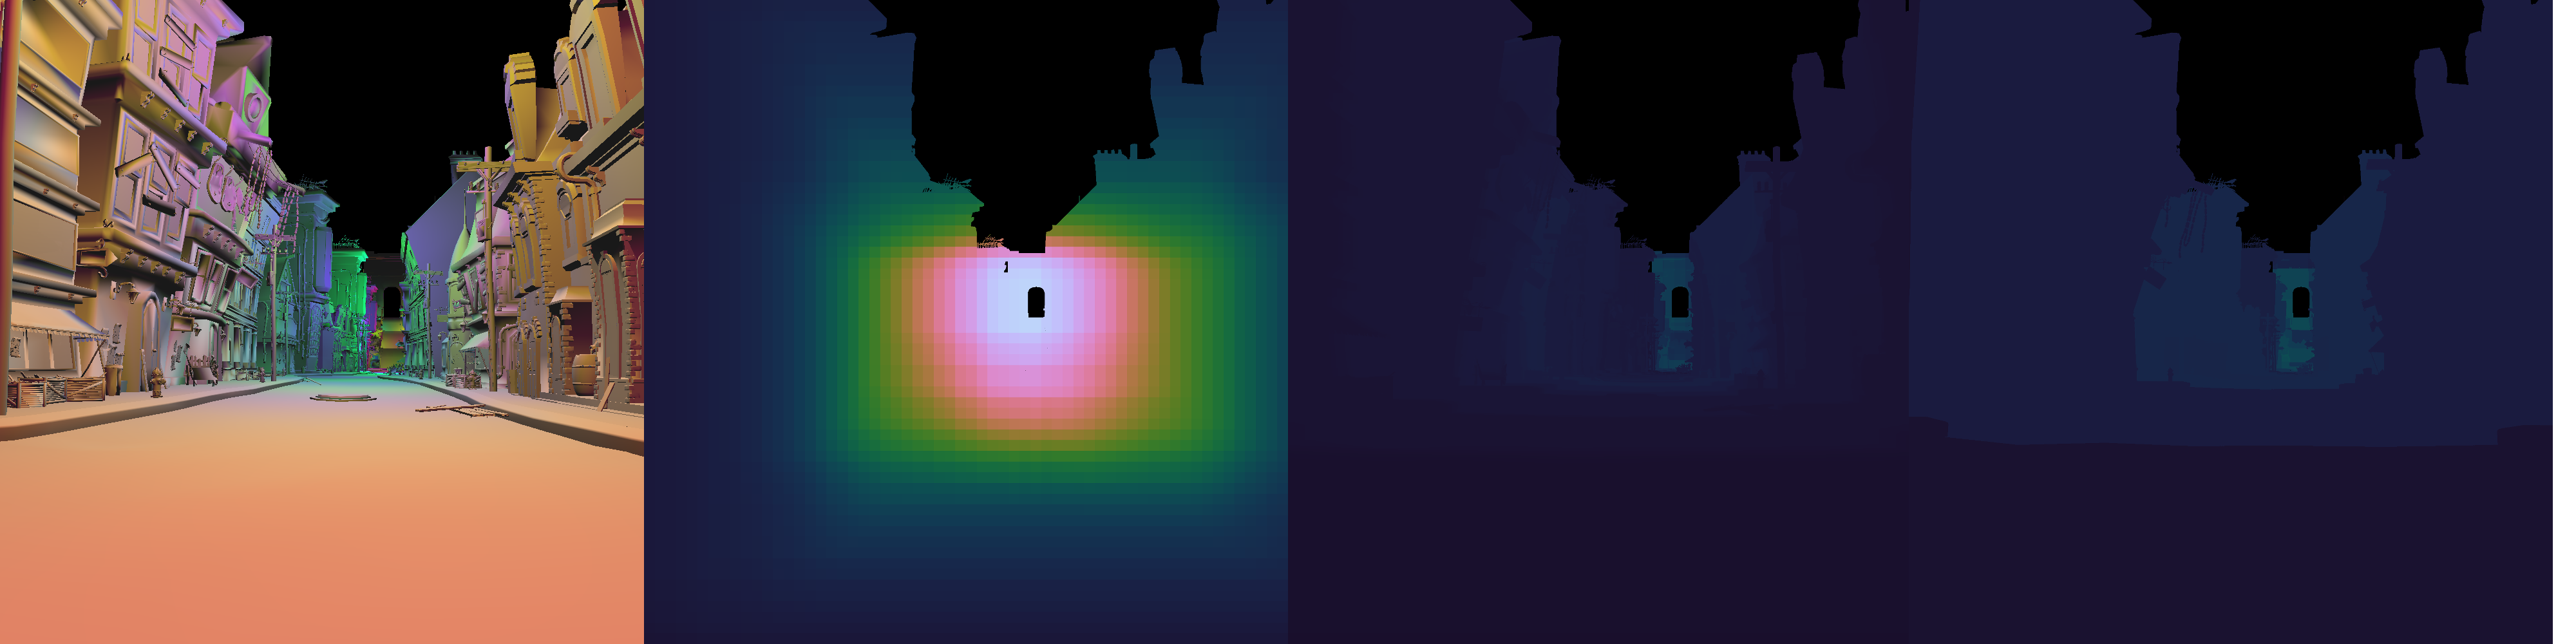
\includegraphics[width=\textwidth]{./img/raw/teaser/teaser.png}
   \caption{The number of light calculations required to shade the image left, for respectively Tiled, Clustered and Hashed Shading.}
   \label{fig:teaser}
\end{teaserfigure}

\begin{abstract}

In this sample paper, we describe the formatting requirements for
content accepted to SIGGRAPH-sponsored events. The same format can be
used for content ranging from a one-page Poster or Talk abstract, to a
full-length Technical Paper. Please review this document even if you
have submitted content to a SIGGRAPH-sponsored event in the past, as
some of the details have changed relative to previous years.

\end{abstract}


\maketitle

\section{Introduction}

In order to push the limits of visual fidelity, modern games are shaded with
ever increasing number of lights and shaders with more complexity. These shading
calculations make up a significant percentage of the amount of work to render a
single frame. To facilitate these complex shading calculations in a real-time
application, it is important that the number of light calculations is kept to
a minimum. There are several different approaches to reducing this workload.
Light assignment in one of such approaches. It is a technique that reduces the
number of light calculations per pixel be excluding lights that do not influence
a pixel. This is possible due to representing lights as having a finite volume
of influence. Ideally, per pixel only lights which are contained in the light
volume are evaluated for that pixel.

In modern games two light assignment algorithms are used commonly. Tiled
Shading\cite{} and Clustered Shading\cite{}. Both rely on a subdivision
of the view frustum to assign lights to pixels. This requires a complete
recalculation of the associated data structures per frame. With a high frame
rate of between 30 and 60 frames a second, most changes between frames are small
and local. Thus a significant part of the light assignment data structures could
potentially be reused.

We introduce the Hashed Shading algorithm, which does not require a complete
rebuild of the associated data structures per frame, in order to explore
whether reusing data structures per frame is a feasible approach that leads
to a performance gain compared to Tiled and Clustered Shading.

We make use of a camera-independent octree data structure to subdivide the scene
space. This camera-independent data structure allows us to reuse the data structures
between frames, even if the camera position changes.


\section{Related Work}

\subsection{Deferred Shading}

A first step into reducing the number of light calculations is decoupling
geometry and shading complexity. In the modern graphical pipeline, all geometry
in the view-frustum generates samples, regardless of whether it is occluded.
These samples are shaded and only after shading the visible samples are
determined in the per-pixel operations. In order to just shade the visible
samples, the visibility of the samples has to be determined before shading.
This concept was introduced in hardware design in 1988\cite{} and is called
Deferred Shading. In 1990 a general purpose strategy was introduced based on so
called GBuffers\cite{}. The idea is to render all attributes needed to shade a
sample into texture buffers the size of the screen. Then in a second, deferred
step these values are retrieved from the buffers to calculate the shading
contribution.

A first light assignment approach is to rasterise the light volumes, and
only calculate the contribution of the light for the generated samples.
This technique is called the stencil-optimalisation\cite{}. This reduces
the number of light calculations, as no longer for each sample each light
has to be evaluated, however there are two also two disadvantages of this
optimalisation. Firstly it requires a significant number of memory
accesses, as for each generated sample, the GBuffers have to be sampled.
Secondly the light contributions are accumulated in a buffer, thus leading
to small rounding errors.

\subsection{Tiled Shading}

Tiled Shading was designed to alleviate the memory bandwidth bottleneck of
Deferred Shading with the stencil-optimalisation. The concept is to divide
the screen space into tiles of $\mathit{n} \times \mathit{n}$ pixels. For
each tile the light indices of the overlapping light volumes are stored.
The tiles are subsequently used to determine the set of relevant lights per
sample by retrieving the set of light indices associated with the tile the
sample falls within. This technique thus only requires a single memory access
per sample, instead of a memory access per light, thus reducing the memory
bandwidth significantly.

The tiles can be constructed by projecting the light volumes on the view port
and determining with which tiles it overlaps. The corresponding light index
is added to each of these tiles. A further optimalisation is to reduce the
tile volume by only considering lights that fall within the minimum and
maximum $z$-value of the tile. Any light that does not overlap with this
sub frustum, is not added to the tile.

This technique has been implemented in a number of games\cite{} and game engines\cite{}, including
the unreal engine\cite{}, the frostbyte engine\cite{} and unity\cite{}.

\subsection{Clustered Shading}

Clustered Shading\cite{} extends Tiled Shading by subdividing the space associated
with each tile further. The tiles are subdivided exponentially in the camera
$z$-axis to gain cube-like sub frustums. For each of the sub frustums containing
geometry, the overlapping lights are calculated. Furthermore additional
attributes like normals can be used to create even more precise light assignment.

The subdivision is constructed by first determining the set of clusters which
contain geometry. This is done by transforming the depth buffer in a cluster
buffer, by assigning each sample to a distinct bin. Then the unique clusters
are obtained by locally sorting and compacting each tile. The cluster buffer
is then used to create a mapping from each sample to the unique cluster to
which it belongs. For each of the unique clusters the overlapping lights
are added to construct a set of light indices.

During the shading step the set of light indices is retrieved using the
sample to cluster mapping constructed during the construction of the data
structures. For each of these lights the contributions is calculated and
summed similarly to Tiled Shading.

Clustered Shading is used in several modern games, including in the Avalance
game engine, on which games as Just Cause 2 and 3\cite{} and Doom 4\cite{} are build.

\subsection{Perfect Spatial Hashing}

In order to efficiently subdivide the scene space without using a large amount
of memory an octree data structure is used. A straightforward implementation
using pointers would require a large number of control structures. Control structures
can lead to a significant performance loss on the GPU\cite{}. Thus such using such
an octree would not be feasible in a light assignment algorithm. A different
approach is needed. The linkless octree\cite{} data structure used within this paper
is based upon perfect spatial hash functions\cite{}.

Hash functions can be used to map sparse data $D$ on to a compact memory table $H$.

\begin{equation*}
  D\left(\mathbf{p}\right) = H\left[ \mathit{h}\left(\mathbf{p} \right) \right]
\end{equation*}

\noindent When a hash function is perfect no keys map to the same address. 
This feature can be used on the GPU as it will ensure no control structures are needed to extract a
value associated with a key from memory.

The goal of perfect spatial hashing to hash multi-dimensional sparse data onto a compact
memory table, without having any collisions and maintaining spatial coherence.
This makes the data structure fitted for applications on the graphics card.
The perfect spatial hash function $\mathit{h}$ is build with two imperfect hash functions,
$\mathit{h}_0$ and $\mathit{h}_1$ and an offset hash table $\Phi$. The idea is to dissolve
collisions in $\mathit{h}_0$ with the offset values in $\Phi$. This leads to the following
definition:

\begin{equation*}
  \mathit{h}\left(\mathbf{p}\right) = \mathit{h}_0\left(\mathbf{p}\right) + \Phi\left[\mathit{h}_1\left(\mathbf{p}\right)\right]
\end{equation*}

\noindent where $\mathit{h}_0$ and $\mathit{h}_1$ are simple hash functions defined as:

\begin{align*}
  \mathit{h}_0\left(\mathbf{p}\right) =& \mathbf{p} \operatorname{mod} \dot{m} \\
  \mathit{h}_1\left(\mathbf{p}\right) =& \mathbf{p} \operatorname{mod} \dot{r}
\end{align*}

\noindent where $\dot{m}$ is the dimension of hash table $H$ and $\dot{r}$ the dimension
of hash table $\Phi$.

This representation makes it possible to represent sparse three dimensional data efficiently
in memory. The linkless octree data structure will be build with these perfect spatial hash
functions.

\subsection{Linkless Octree}

The linkless octree is a GPU efficient octree implementation, which is utilised in the
Hashed Shading algorithm. It represents each layer of the octree as a perfect spatial
hash function.

An octree contains a number of layers, each layer has a defined node size, thus the position
of each node can be represented by a three dimensional integer vector. There exists a node
at position $\mathbf{p}_l$ in layer $\mathit{l}$ if and only if at layer $\mathit{l} - 1$
there is a branch node containing the node at position $\mathbf{p}_l$ or $\mathbf{p}_l$ is the
root node of the octree. This means that each layer consists of a set of nodes sparsely distributed
over the octree space. Each layer can thus be efficiently represented by a perfect spatial hash function.

In order to encode a layer, the data associated with a node needs to be defined. This data encodes
the type of an octree node at position $\mathbf{p}$. An octree node can either be a branch
node or a leaf node, and an octree node can be either empty or non-empty. Thus each octree node
can be represented by two boolean values. Due to memory considerations eight nodes are combined
and represented by two 8-bit integers. Since each branch node contains eight children, each
linkless octree node in layer $\mathit{l}$ represents a branch node containing the types of
its eight children at depth $\mathit{l}+1$.
A complete octree can be represented by constructing a perfect spatial hash function for each
layer.

The data saved in the octree node needs to be stored as well. There are two options to do this.
Either the data is stored directly in the hash table of the perfect spatial hash function, or
the data is stored separately. In case the data is stored directly inside the hash table,
each hash table entry requires the memory to hold two 8-bit integers and eight times the
memory of a single data element associated with an octree node. This approach is infeasible
when the data is large, or only a small subset of nodes actually contains data. In these
cases the data can be saved in a separate perfect spatial hash function. The hash table
associated with this second perfect spatial hash function will contain an entry for each non-empty
child node of the nodes saved in the first spatial hash function.

  
\section{Hashed Shading Algorithm}
%\subsection{Overview}

\begin{figure}[t]
  \usetikzlibrary{shapes.arrows, fadings}
  \definecolor{LightColor}{rgb}{1.0,0.901,0.805}

  \definecolor{tile0}{HTML}{DABDE4}
  \definecolor{tile1}{HTML}{B8DBF4}
  \definecolor{tile2}{HTML}{B5EDCD}
  \definecolor{tile3}{HTML}{FBEBA7}
  \definecolor{tile4}{HTML}{F9C1BB}
  \definecolor{tile5}{rgb}{1, 1, 1}

  \tikzstyle{array_element}=[rectangle,
                             minimum height=1cm, 
                             minimum width=1cm, 
                             minimum size=1cm,
                             draw=black,
                             rounded corners=2.5 ]
  \tikzstyle{grid_element}=[rectangle,
                            minimum height=1.5cm, 
                            minimum width=1.5cm, 
                            draw=black,
                            rounded corners=2.5 ]
  \tikzstyle{grid_element_big}=[rectangle, 
                               minimum height=2cm, 
                               minimum width=2cm, 
                               draw=black,
                               rounded corners=2.5 ]
 \tikzstyle{grid_element_bigly}=[rectangle, 
                               minimum height=3cm, 
                               minimum width=3cm, 
                               draw=black,
                               rounded corners=2.5 ]


\begin{adjustbox}{minipage=\textwidth, scale=0.5}
  \centering
  \begin{tikzpicture}
    \node at (-4.cm, 4cm) (light_list_name) [anchor=west] {\LARGE Global Light List:};
    \node at (-4.cm, 2cm) (light_list_name) [anchor=west] {\LARGE Light Index List:};
    \node at (-4.cm, -1.5cm) (light_list_name) [anchor=west] {\LARGE Octree:};
    \node at (2.75cm, -1.5cm) (light_list_name) [anchor=west] {\LARGE Spatial Hash Functions:};
    

    \foreach \l in {0,...,6} {
      \node at (1cm * \l + 1cm, 4cm) (light_\l) [array_element,fill={LightColor}] {$\mathbf{l}_\l$};
    }
    \node at (1cm * 7, 4cm) [array_element, fill={LightColor}, ] {};
    \node at (1cm * 7.325, 4cm) [rectangle,
                                 minimum height=1.2cm,
                                 minimum width=0.6cm,
                                 fill={white},
                                 draw=white] {};
    \node at (1cm * 7, 4cm) [rectangle,                    
                             minimum height=0.98cm, 
                             minimum width=0.2cm, 
                             shading = axis,
                             shading angle=90,
                             left color=LightColor ] {};
                             
    \node at (1cm * 7, 4cm) [rectangle, minimum height=1cm, minimum width=1cm] {$\dots$};

    \node at (1cm * 0, 2cm) [array_element,
                              fill={white}, ] {};
    \node at (1cm * -0.325, 2cm) [rectangle,
                                  minimum height=1.2cm,
                                  minimum width=0.6cm,
                                  fill={white},
                                  draw=white] {};
    \node at (1cm * 0, 2cm) [rectangle,
                              minimum height=1cm,
                              minimum width=1cm] {$\dots$};


    \foreach \i/\l in {0/0} {
      \node at (1cm * \i +1cm, 2cm) (light_index_\i) [array_element, fill={tile0}] {\l};
      \draw[-latex] (light_index_\i.north) -- (light_\l.south);
    }
    \foreach \i/\l in {1/0, 2/1, 3/4} {
      \node at (1cm * \i  +1cm, 2cm) (light_index_\i) [array_element, fill={tile1}] {\l};
      \draw[-latex] (light_index_\i.north) -- (light_\l.south);
    }
    \foreach \i/\l in {4/2, 5/4} {
      \node at (1cm * \i  +1cm, 2cm) (light_index_\i) [array_element, fill={tile2}] {\l};
      \draw[-latex] (light_index_\i.north) -- (light_\l.south);
    }
    \foreach \i/\l in {6/5} {
      \node at (1cm * \i  +1cm, 2cm) (light_index_\i) [array_element, fill={tile3}] {\l};
      \draw[-latex] (light_index_\i.north) -- (light_\l.south);
    }
    \foreach \i/\l in {7/3, 8/5, 9/6} {
      \node at (1cm * \i  +1cm, 2cm) (light_index_\i) [array_element, fill={tile4}] {\l};
      \draw[-latex] (light_index_\i.north) -- (light_\l.south);
    }
    \node at (1cm * 10  +1cm, 2cm) [array_element,
                              fill={white}, ] {};
    \node at (1cm * 10.325  +1cm, 2cm) [rectangle,
                                  minimum height=1.2cm,
                                  minimum width=0.6cm,
                                  fill={white},
                                  draw=white] {};
    \node at (1cm * 10  +1cm, 2cm) [rectangle,
                              minimum height=1cm,
                              minimum width=1cm] {$\dots$};

\node[inner sep=0pt] (level_0) at (-1.25cm,-5.5cm - 1cm)
    {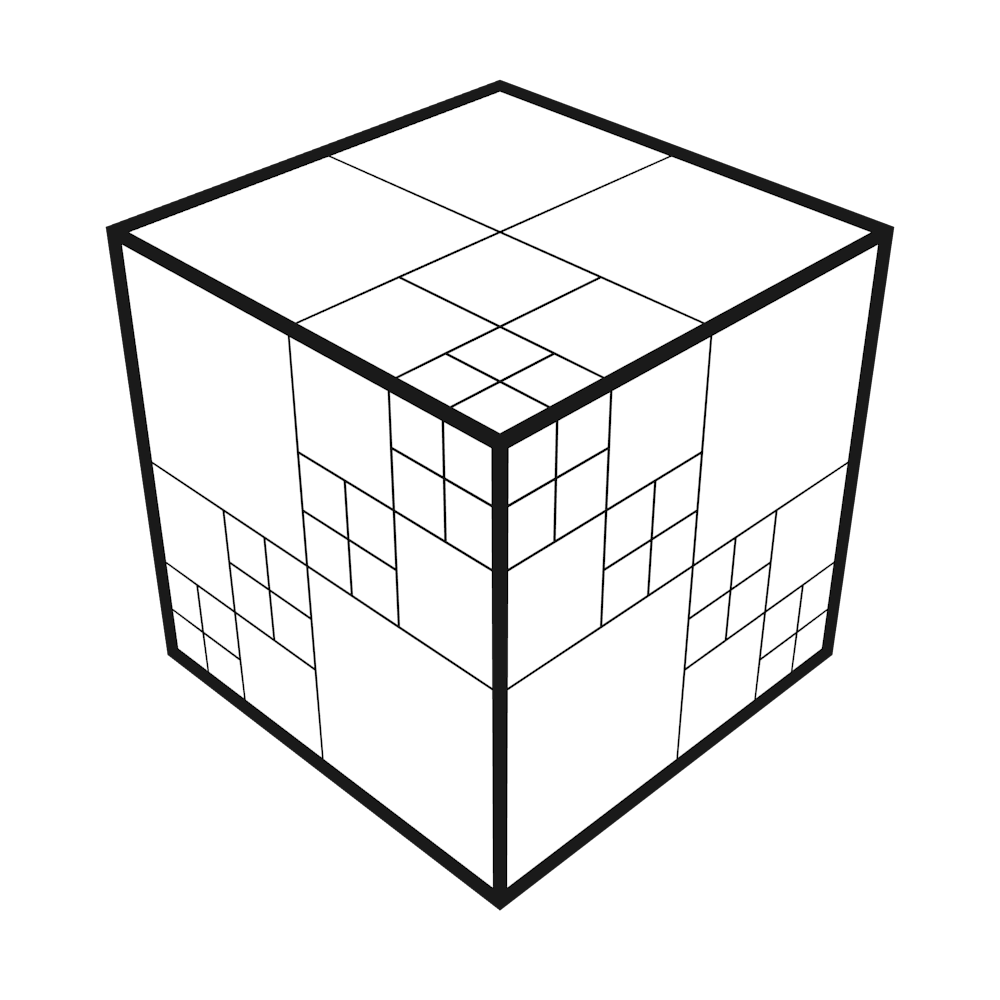
\includegraphics[width=6.5cm]{./img/raw/hs-datastructuren-overzicht/octree.png}};
    
\node at (4cm, -2.cm) {$\vdots$};
\node at (4cm, -10.5cm) {$\vdots$};




\node[inner sep=0pt] (level_0) at (4.0cm,-3cm  - 1.5cm)
    {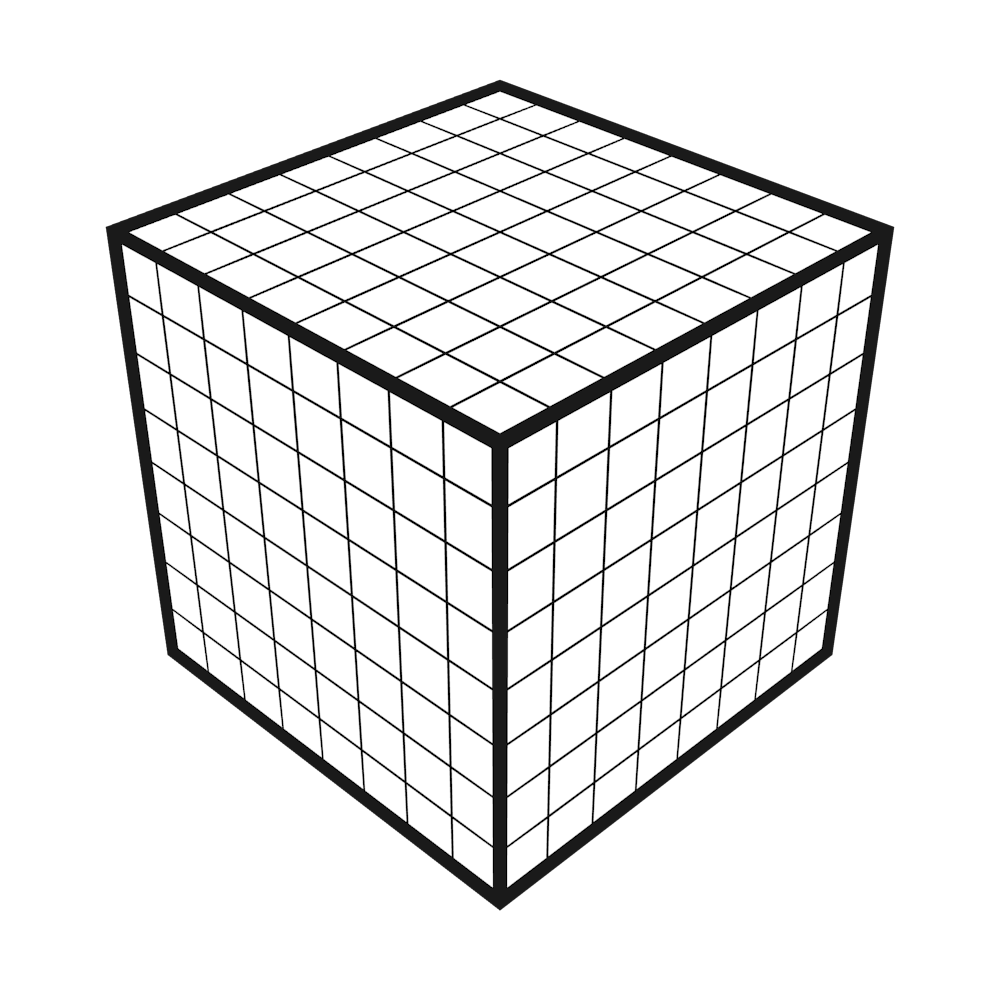
\includegraphics[width=3cm]{./img/raw/hs-datastructuren-overzicht/img1.png}};
\node[inner sep=0pt] (level_0) at (6.25cm,-2.75cm  - 1.5cm)
    {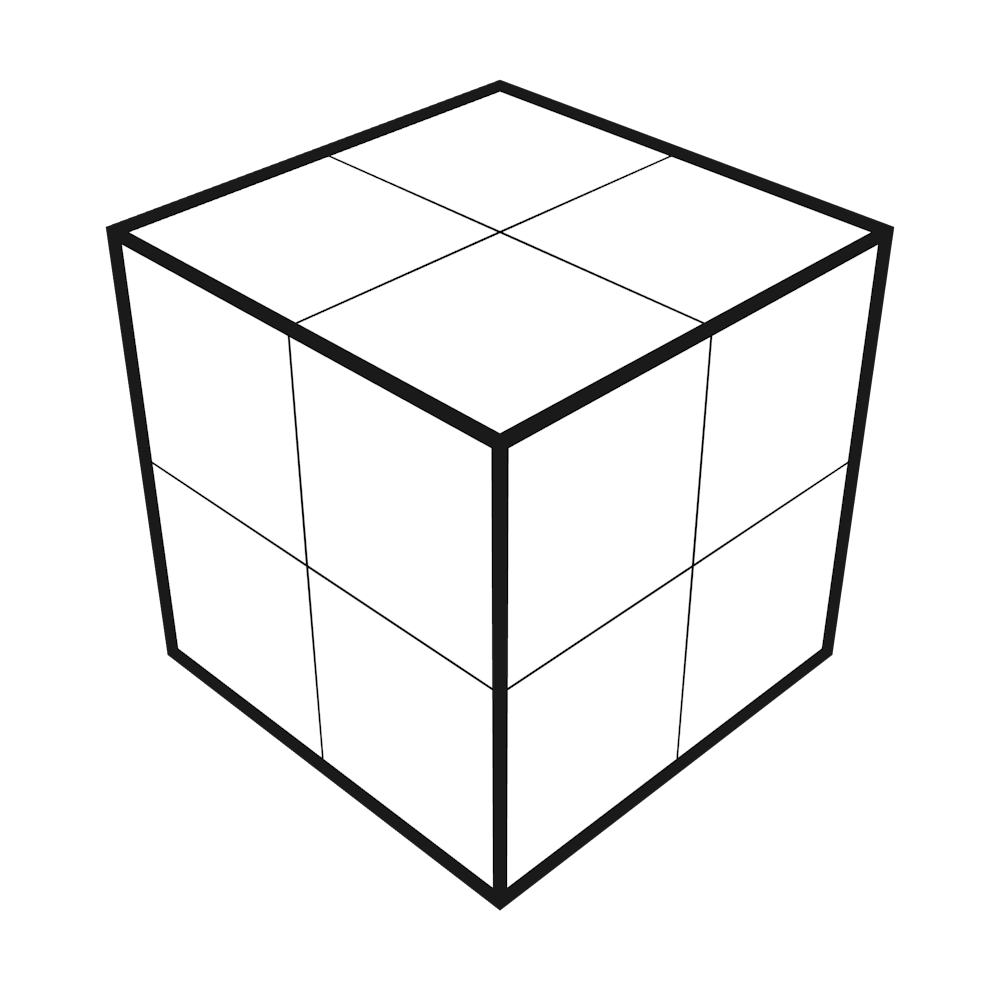
\includegraphics[width=2cm]{./img/raw/hs-datastructuren-overzicht/img2.png}};
\node[inner sep=0pt] (level_0) at (8.5cm,-3cm  - 1.5cm)
    {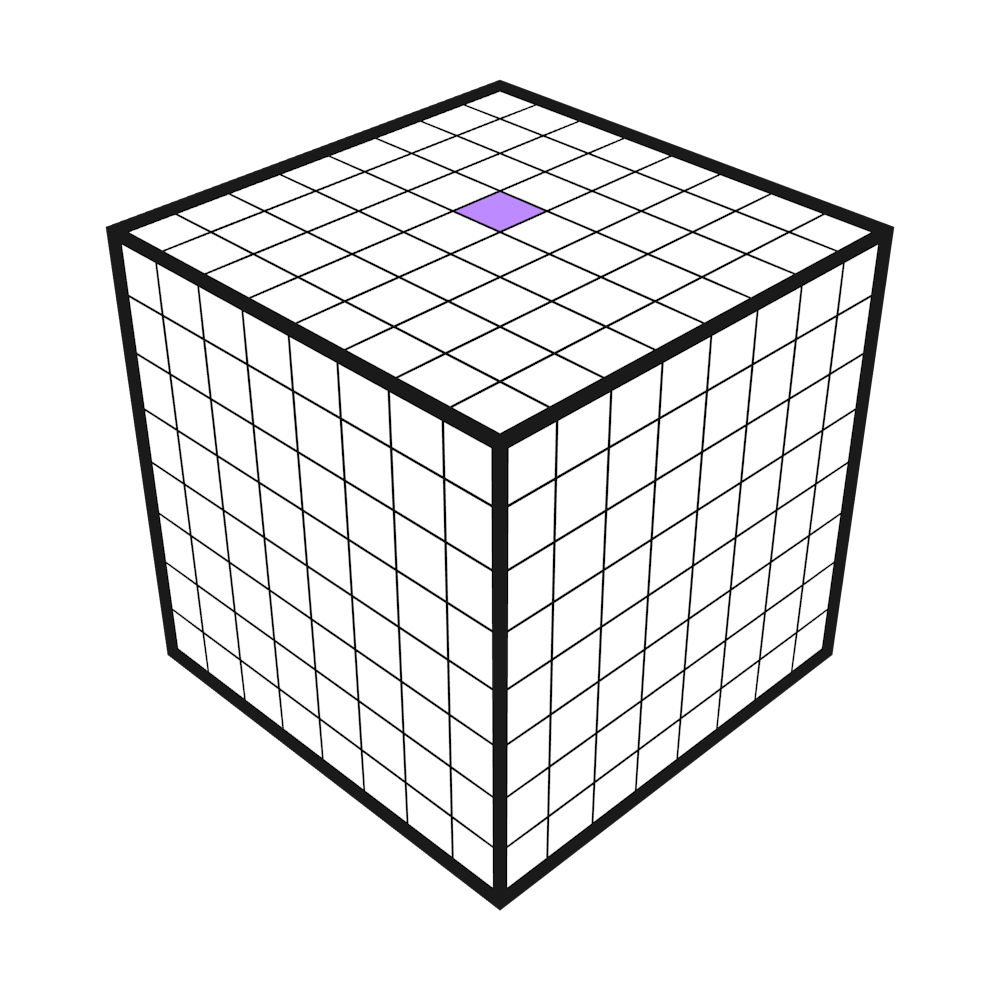
\includegraphics[width=3cm]{./img/raw/hs-datastructuren-overzicht/img3.png}};
\node[inner sep=0pt] (level_0) at (10.75cm,-2.75cm  - 1.5cm)
    {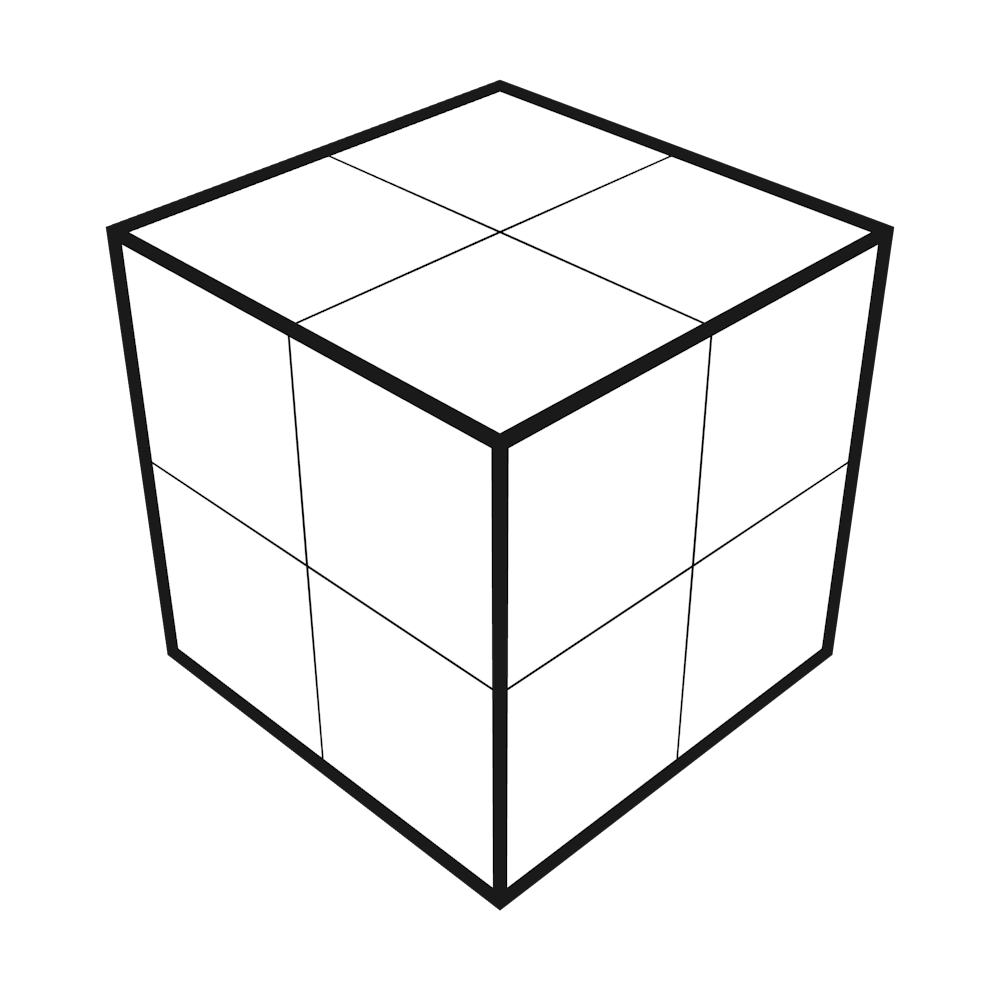
\includegraphics[width=2cm]{./img/raw/hs-datastructuren-overzicht/img2.png}};

\node[inner sep=0pt] (level_0) at (4.0cm,-3cm - 3.75cm  - 1.5cm)
    {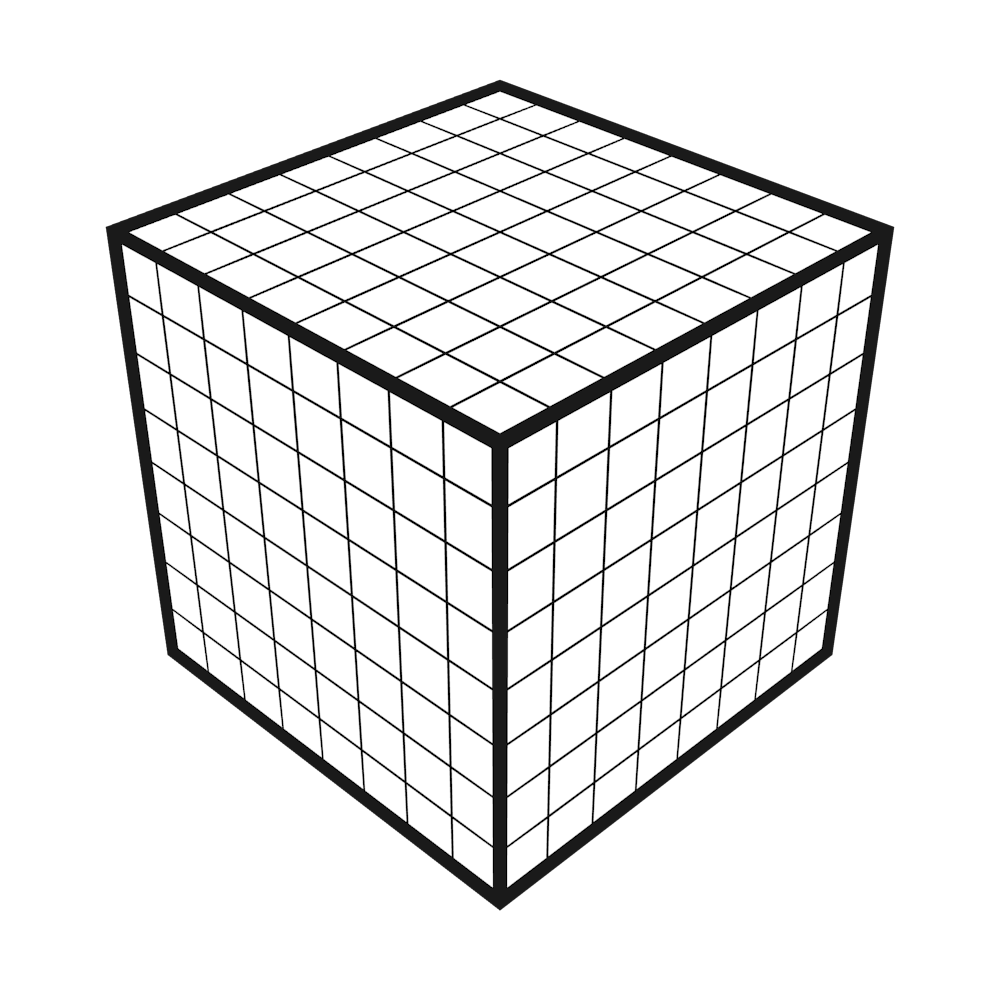
\includegraphics[width=3cm]{./img/raw/hs-datastructuren-overzicht/img1.png}};
\node[inner sep=0pt] (level_0) at (6.25cm,-2.75cm - 3.75cm  - 1.5cm)
    {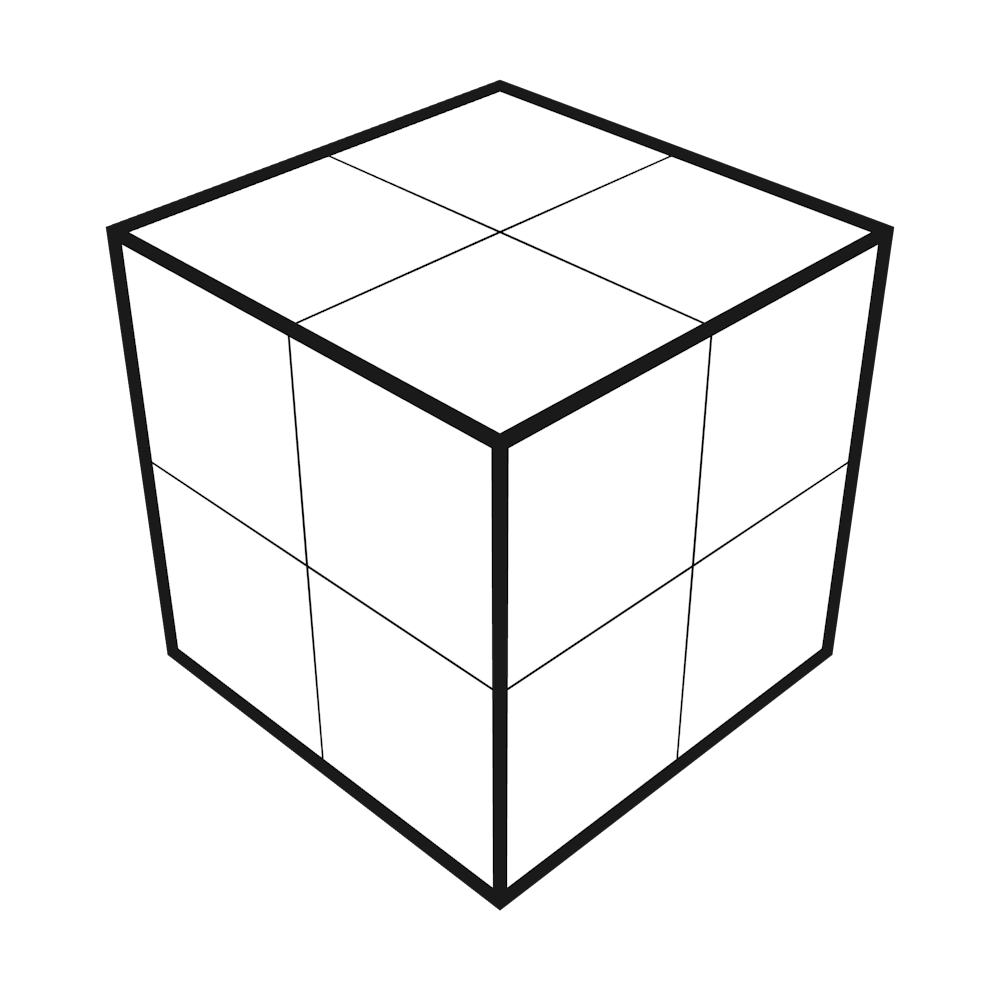
\includegraphics[width=2cm]{./img/raw/hs-datastructuren-overzicht/img2.png}};
\node[inner sep=0pt] (level_0) at (8.5cm,-3cm - 3.75cm  - 1.5cm)
    {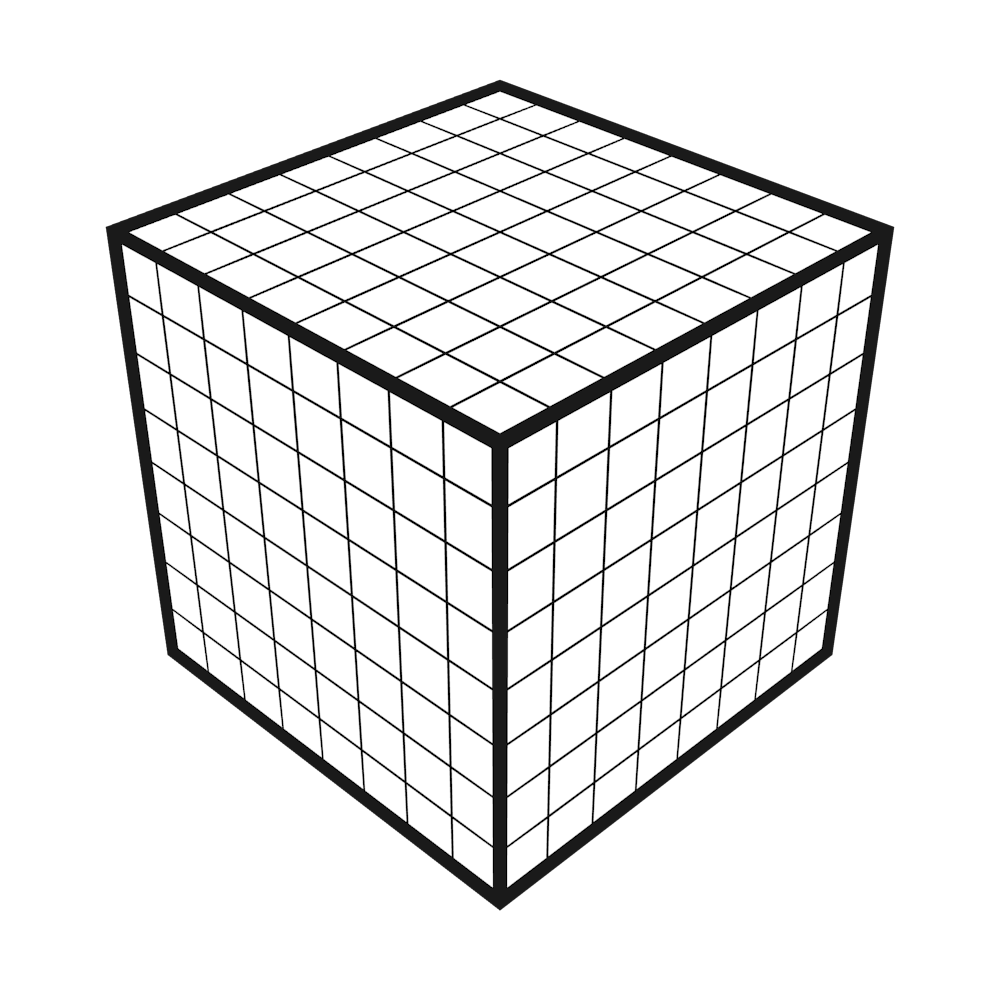
\includegraphics[width=3cm]{./img/raw/hs-datastructuren-overzicht/img1.png}};
\node[inner sep=0pt] (level_0) at (10.75cm,-2.75cm - 3.75cm  - 1.5cm)
    {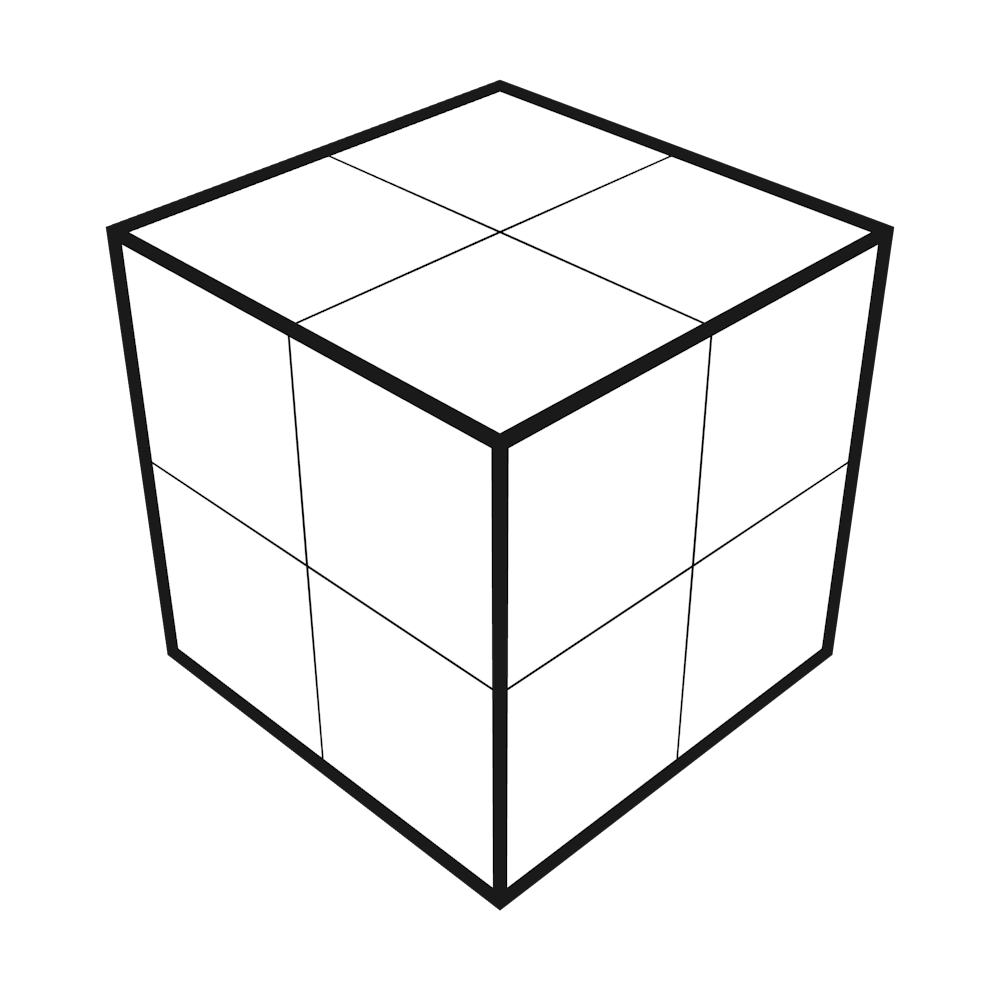
\includegraphics[width=2cm]{./img/raw/hs-datastructuren-overzicht/img2.png}};

\node at (11.75cm, -2.8cm) {\scriptsize layer $i$};
\node at (11.75cm, -2.8cm - 3.75cm) {\scriptsize layer $i + 1$};

\node at (3.0cm, -3.25cm) {$H_{1,i}$};
\node at (5.75cm, -3.25cm) {$\Phi_{1,i}$};
\node at (7.5cm, -3.25cm) {$H_{2,i}$};
\node at (10.25cm, -3.25cm) {$\Phi_{2,i}$};

\node at (3.0cm, -3.25cm -3.75cm) {$H_{1,i + 1}$};
\node at (5.75cm, -3.25cm  -3.75cm) {$\Phi_{1,i + 1}$};
\node at (7.5cm, -3.25cm -3.75cm) {$H_{2,i + 1}$};
\node at (10.25cm, -3.25cm -3.75cm) {$\Phi_{2,i + 1}$};

\node at (2cm, -2.5cm) (l1) {};
\node at (12.75cm, -2.5cm) (l2) {};
\draw[-, gray, very thin] (l1) -- (l2);

\node at (2cm, -2.5cm  -3.75cm) (l1) {};
\node at (12.75cm, -2.5cm  -3.75cm) (l2) {};
\draw[-, gray, very thin] (l1) -- (l2);

\node at (2cm, -2.5cm  -3.75cm -3.75cm) (l1) {};
\node at (12.75cm, -2.5cm  -3.75cm -3.75cm) (l2) {};
\draw[-, gray, very thin] (l1) -- (l2);

\node at (8.35cm, -3.63cm) (l1) {};
\node at (8.625cm, -3.63cm) (l2) {};

    \node at (-2.25cm + 10.75cm, -2cm + 1.5cm) (node_big) [grid_element_big, fill=tile0] {};
    \node at (-3.25cm + 10.75cm , -2cm + 1.5cm) (grid_l) [] {};
    \node at (-1.25cm + 10.75cm, -2cm + 1.5cm) (grid_r) [] {};
    \draw (grid_l.center) -- (grid_r.center);
    \node at (-2.25cm + 10.75cm, -1.5cm + 1.5cm) [] { \Large offset: $\mathit{k}$ };
    \node at (-2.25cm + 10.75cm, -2.5cm + 1.5cm) [] { \Large size: $\mathit{1}$ };

    \node at (-3.25cm + 10.75cm, -3cm + 1.55cm) (node_big_1) {};
    \node at (-1.25cm + 10.75cm, -3cm + 1.55cm) (node_big_2) {};


    \draw[gray] (node_big_1.center) -- (l1.center);
    \draw[gray] (node_big_2.center) -- (l2.center);
    
    \draw[-latex] (node_big.west) -- (light_index_0.south);


  \end{tikzpicture}
  \end{adjustbox}

  \caption{Overview of the data structures of Hashed Shading.}
  \label{fig:hs-data-structures}
\end{figure}


The goal of the Hashed Shading algorithm is to reduce the amount of work
required to build the data structures between frames, in order to improve the
overall performance compared to Tiled and Clustered Shading. It does so by
dividing the scene space camera-independently. Thus the data structures can be
reused between frames even if the camera position changes.
The scene space is represented with an octree data structure. This representation
is both precise and memory efficient.

The used data structures are based on the data structured used within Tiled and
Clustered Shading:

\begin{itemize}
  \item Linkless octree
  \item Light index list
  \item Global light list
\end{itemize}

\noindent The linkless octree replaces the tiles and clusters in Tiled and Clustered
Shading respectively. It contains two integers per filled node, one that defines the
offset within the light index list, and one that defines the size of the set of
indices within the light index list.

In order to construct these data structures the following steps have to be executed:

\begin{itemize}
  \item Define the scene space subdivision.
  \item Calculate the influence of each light on the subdivision.
  \item Combine the influences into one single scene octree.
  \item Construct the linkless octree and light index list based on the scene octree.
\end{itemize}

\noindent The first step requires the origin of the octree and the total size to be
calculated. Once these values are specified it is possible to define the influence
of each light in the scene. The combination of these influences leads to a scene
octree which has to be represented as a linkless octree in order to be used
effectively on the GPU. Finally for each sample the set of relevant lights is calculated
by descending into the octree. These steps will be explained in more detail in the
following chapters.

\subsection{Specification of the Octree}

To construct the octree a minimum bounding box which will fit all the lights at any
point in time during the simulation, needs to be defined. The minimum and maximum
points that define this bounding box can either be set by a developer or calculated
based on the light volumes. In order to ensure small rounding errors do not affect
the octree, an offset is added to these points.

Once the bounding box has been defined the size of the octree can be calculated. The
developer is responsible for setting the size of the nodes in the deepest layer of
the octree. Based on this node size $\mathit{l}$, the size of the octree can be calculated.
Assuming that $\mathit{d}_i$ is the maximum length of any of the sides of the
bounding box, the number of layers is equal to the smallest value of $k$ for
which holds

\begin{equation*}
  \mathit{l} \cdot 2^k \geq \mathit{d}_i
\end{equation*}

\noindent The size of the octree is equal to $\mathit{l} \cdot 2^k$.
With the origin and size defined it is possible to assign the lights to this subdivision of
space.

\subsection{Per Light Construction}

\begin{figure}[t]
  \centering
  \begin{subfigure}[b]{.3\linewidth}
    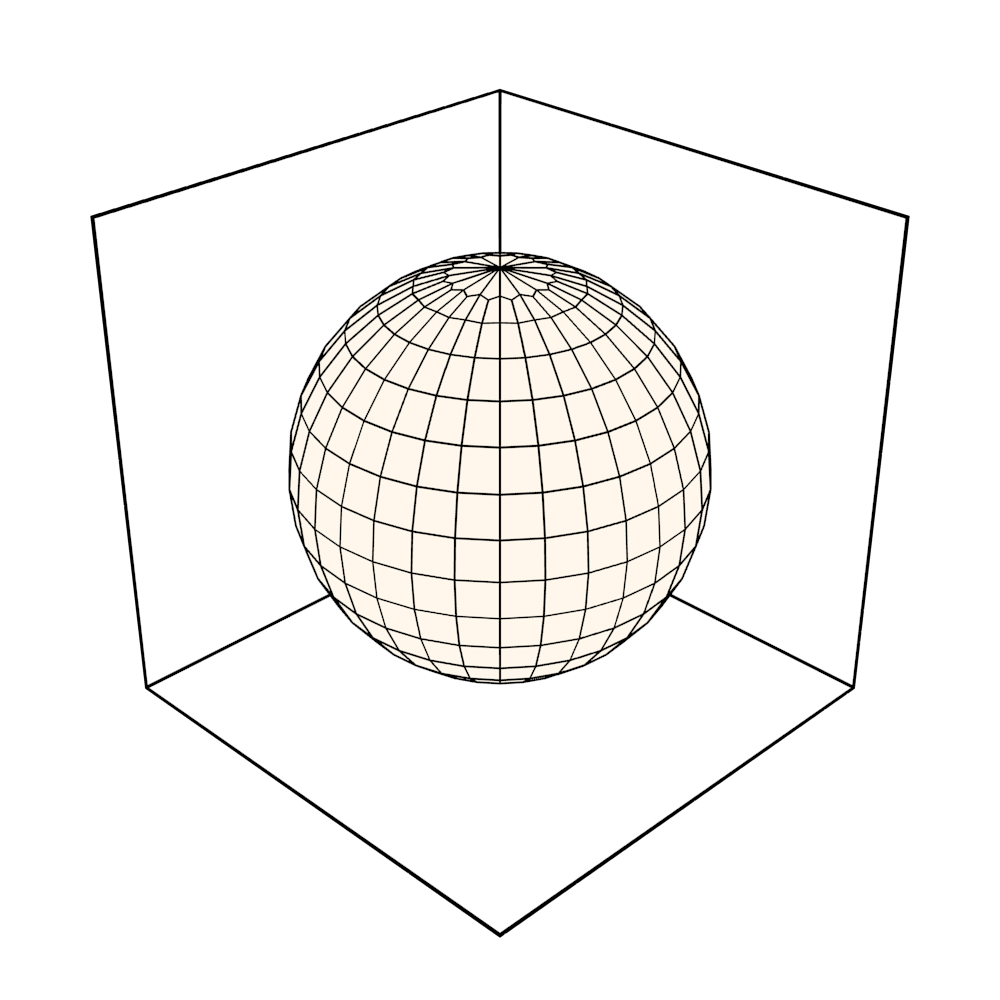
\includegraphics[width=\textwidth]{./img/raw/hs-slt-algorithm/hs-slt-algorithm-1.png}%
    \caption{\footnotesize Initial light volume}%
    \label{fig:hs-p1a}%
  \end{subfigure}
  %
  \begin{subfigure}[b]{.3\linewidth}
    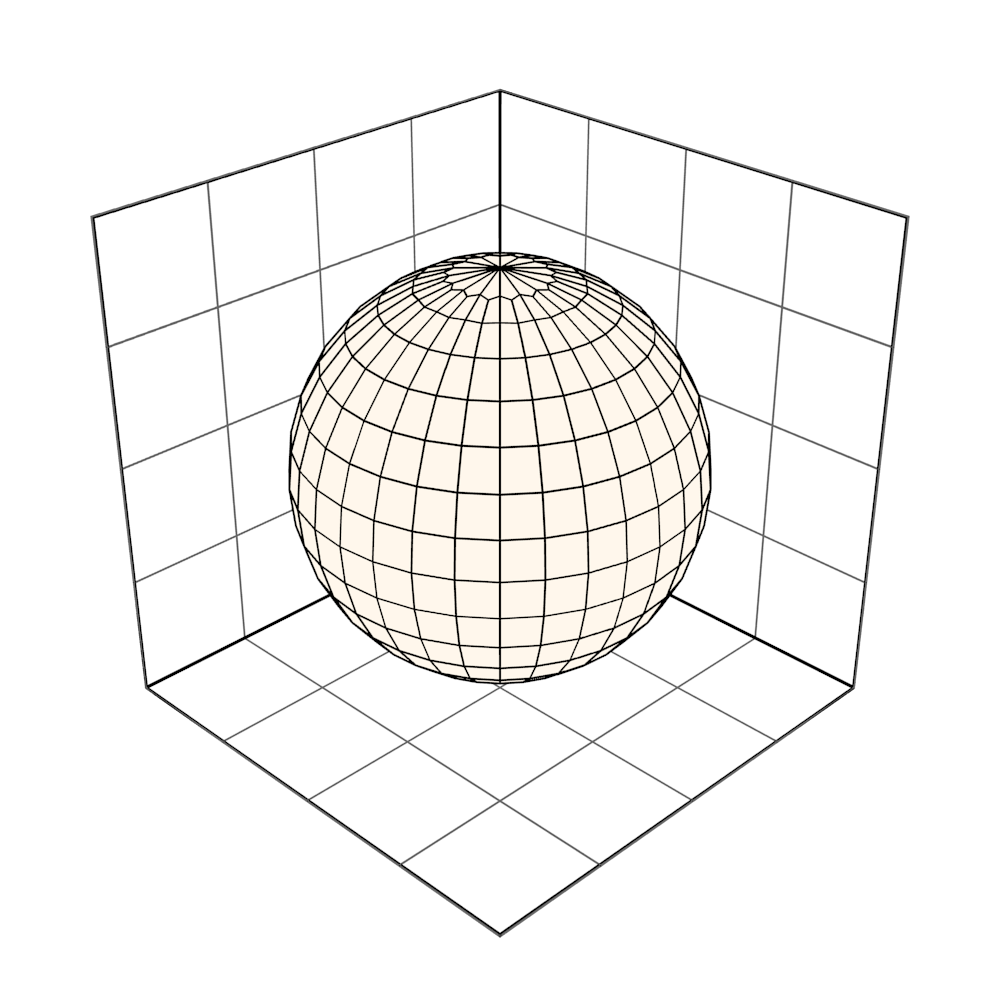
\includegraphics[width=\textwidth]{./img/raw/hs-slt-algorithm/hs-slt-algorithm-2.png}%
    \caption{\footnotesize Define grid}%
    \label{fig:hs-p1b}%
  \end{subfigure}
  %
  \begin{subfigure}[b]{.3\linewidth}
    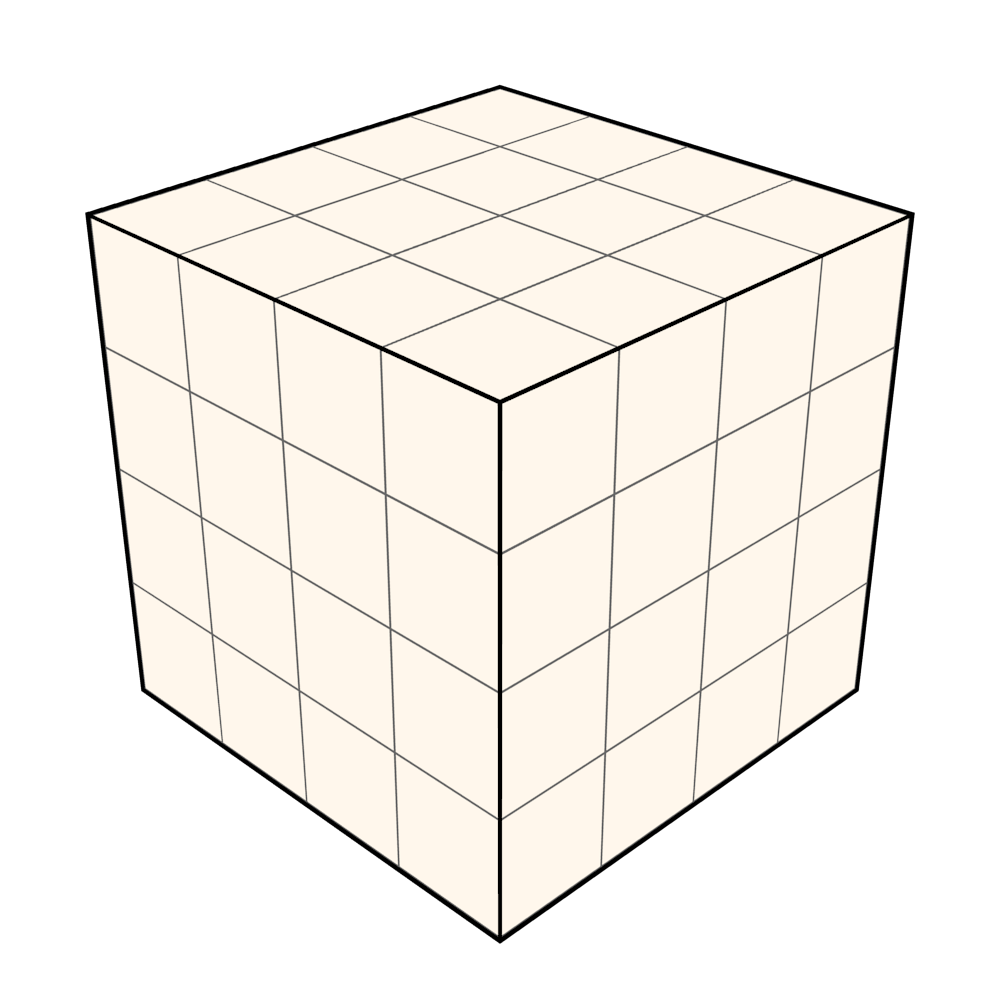
\includegraphics[width=\textwidth]{./img/raw/hs-slt-algorithm/hs-slt-algorithm-3.png}%
    \caption{\footnotesize Initialise grid}%
    \label{fig:hs-p1c}%
  \end{subfigure}
  \\
  \begin{subfigure}[b]{.3\linewidth}
    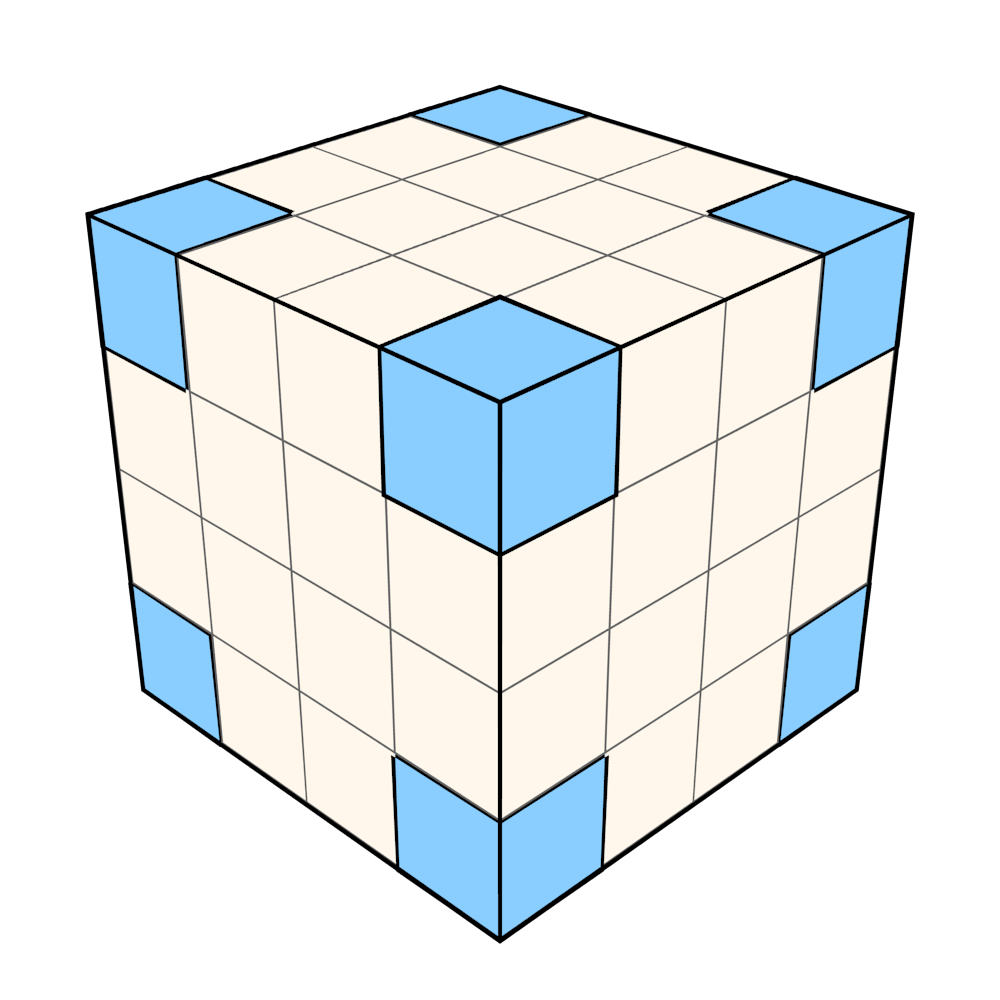
\includegraphics[width=\textwidth]{./img/raw/hs-slt-algorithm/hs-slt-algorithm-4.png}%
    \caption{\footnotesize Evaluate nodes}%
    \label{fig:hs-p1d}%
  \end{subfigure}
  %
  \begin{subfigure}[b]{.3\linewidth}
    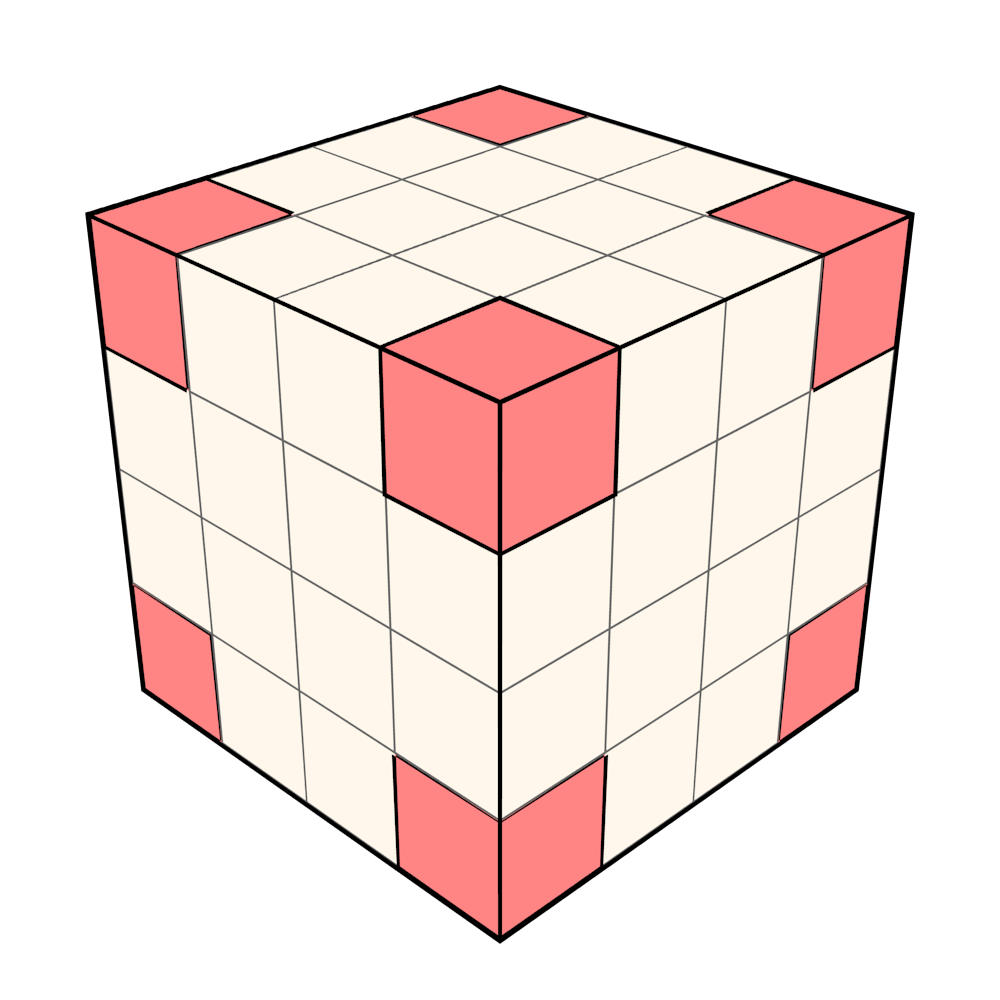
\includegraphics[width=\textwidth]{./img/raw/hs-slt-algorithm/hs-slt-algorithm-5.png}%
    \caption{\footnotesize Mark nodes}%
    \label{fig:hs-p1e}%
  \end{subfigure}
  %
  \begin{subfigure}[b]{.3\linewidth}
    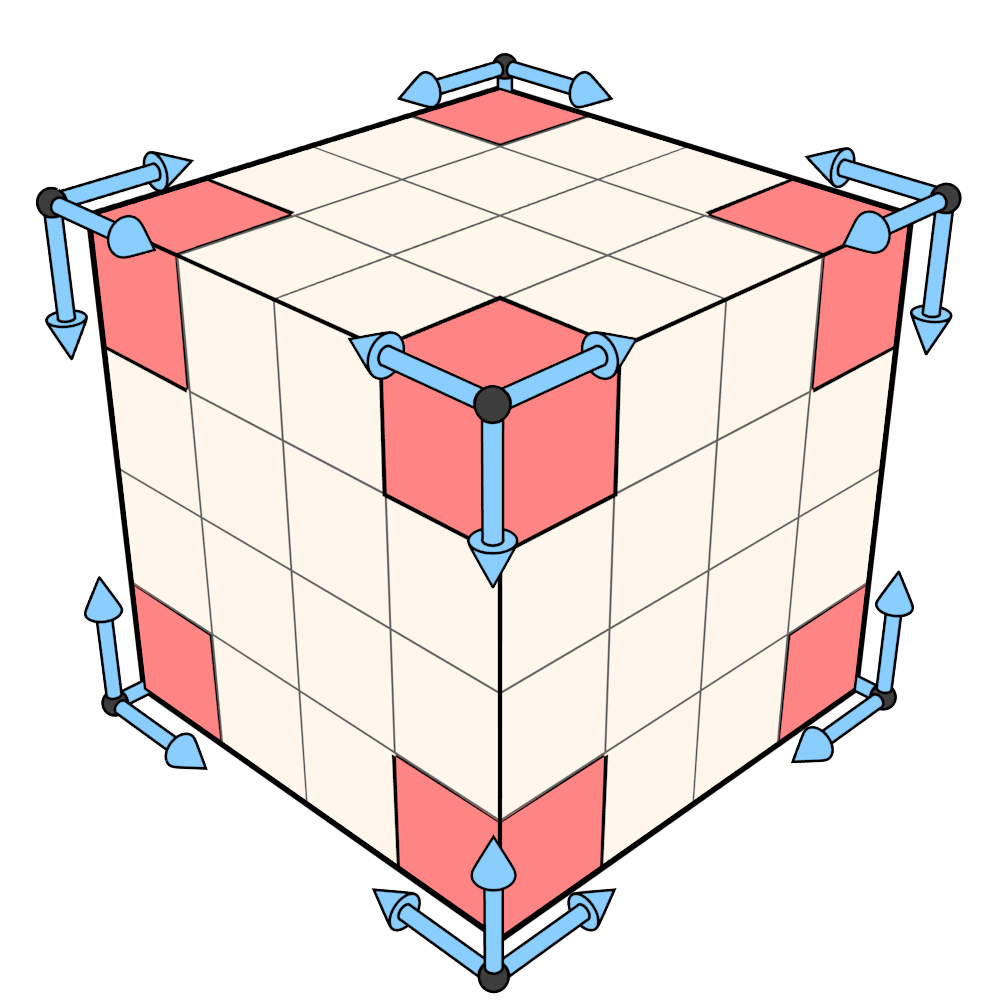
\includegraphics[width=\textwidth]{./img/raw/hs-slt-algorithm/hs-slt-algorithm-6.png}%
    \caption{\footnotesize Select nodes}%
    \label{fig:hs-p1f}%
  \end{subfigure}
  \\
  \begin{subfigure}[b]{.3\linewidth}
    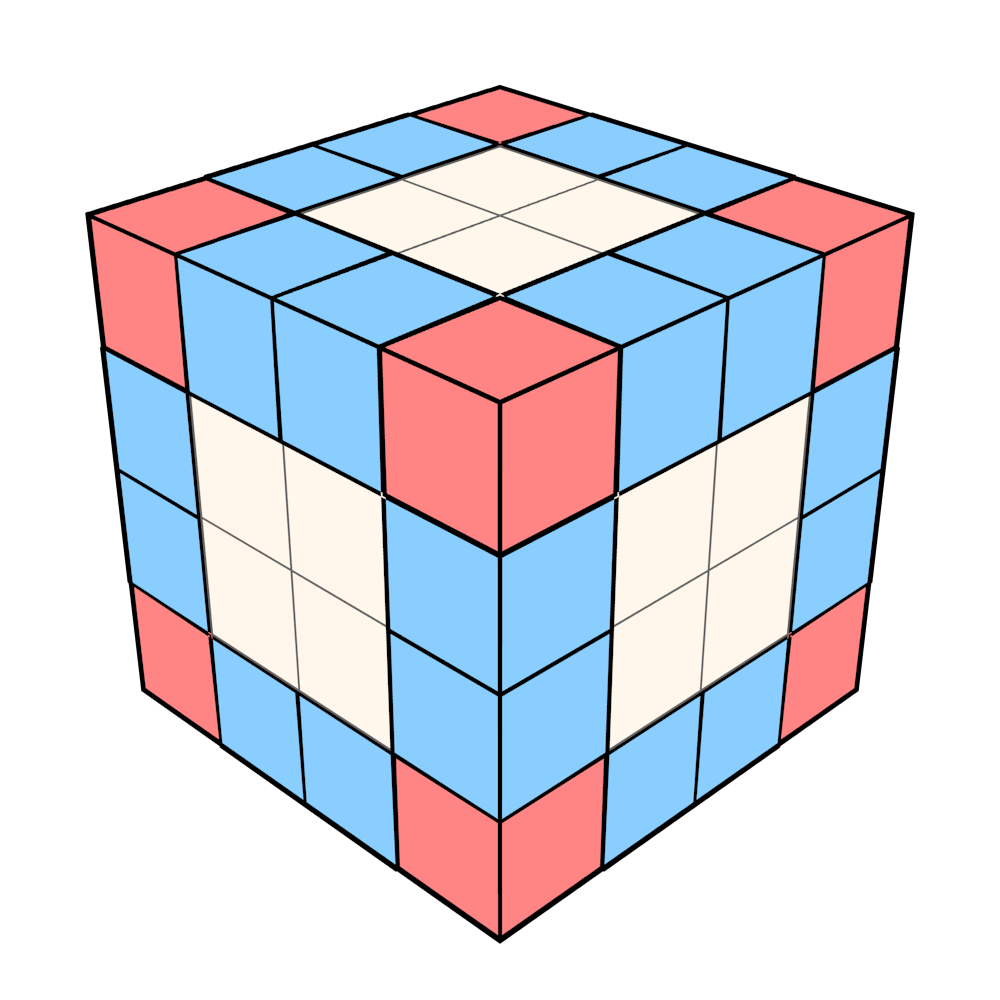
\includegraphics[width=\textwidth]{./img/raw/hs-slt-algorithm/hs-slt-algorithm-7.png}%
    \caption{\footnotesize Evaluate nodes}%
    \label{fig:hs-p1g}%
  \end{subfigure}
  %
  \begin{subfigure}[b]{.3\linewidth}
    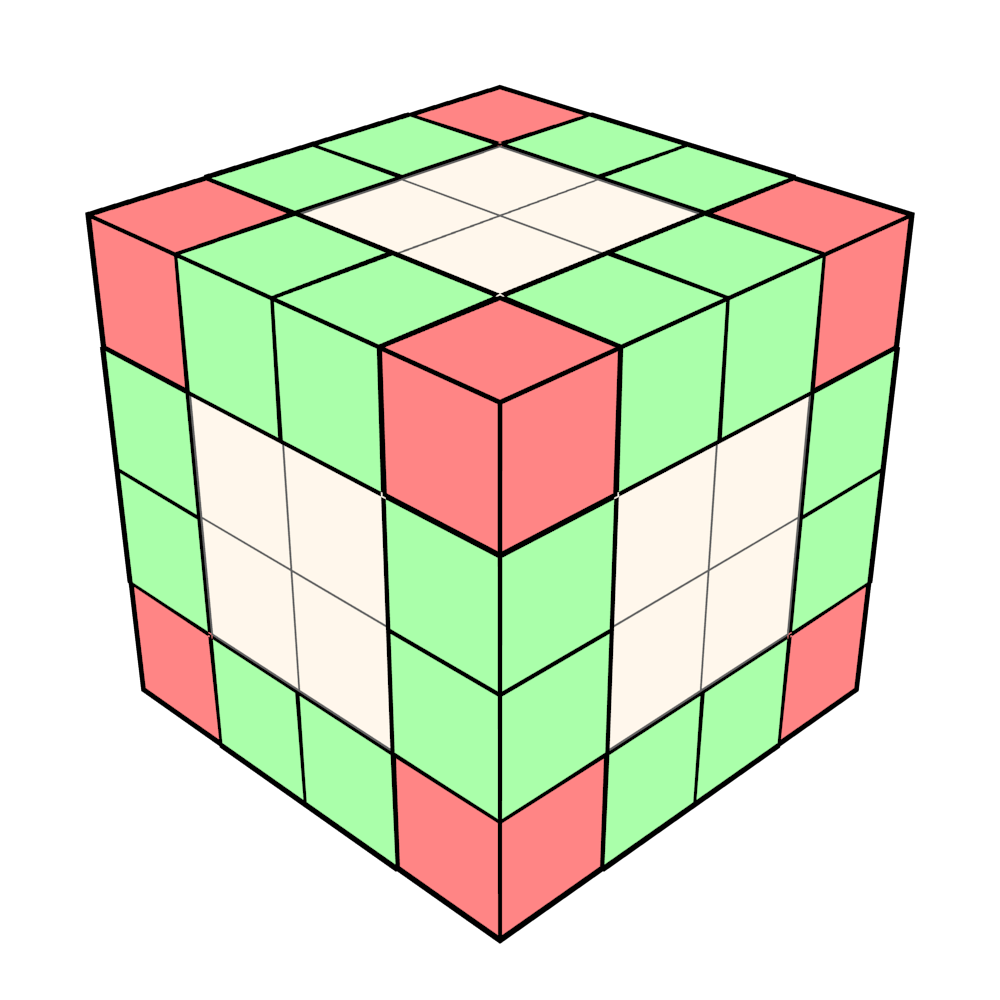
\includegraphics[width=\textwidth]{./img/raw/hs-slt-algorithm/hs-slt-algorithm-8.png}%
    \caption{\footnotesize Mark nodes}%
    \label{fig:hs-p1h}%
  \end{subfigure}
  %
  \begin{subfigure}[b]{.3\linewidth}
    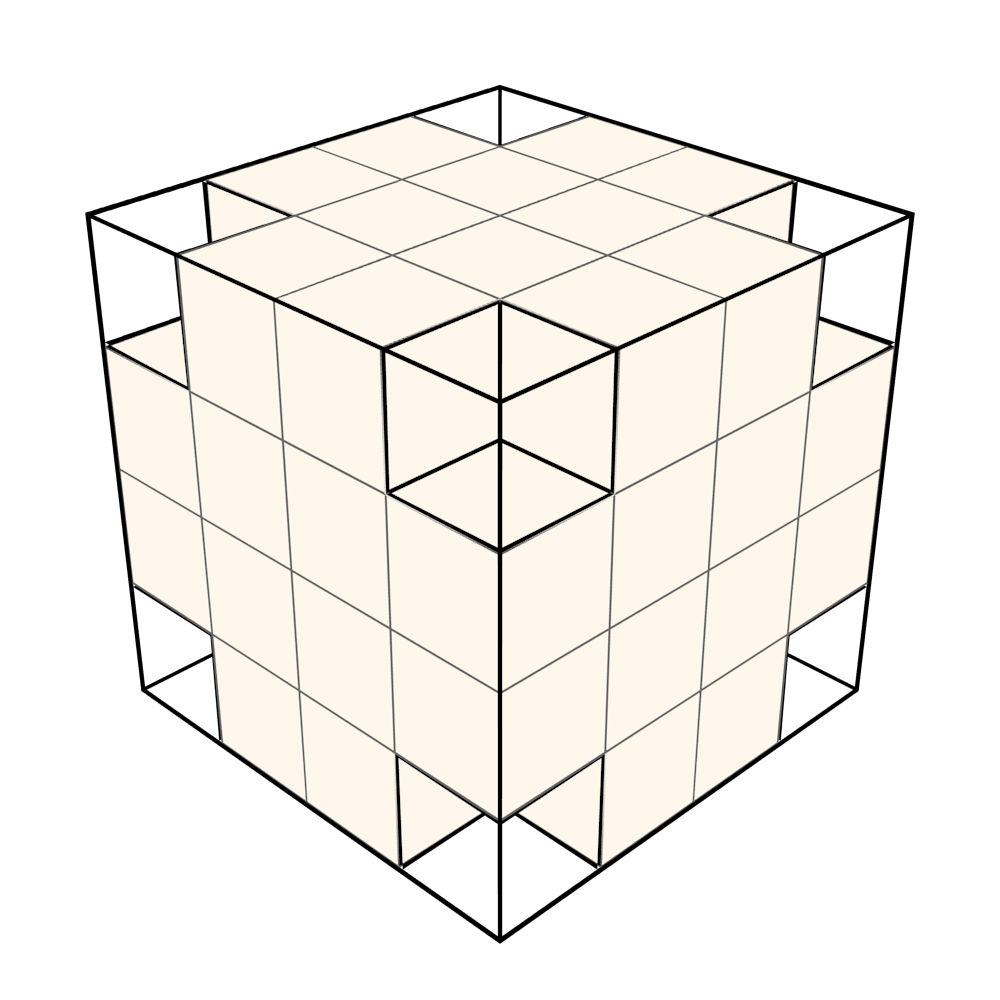
\includegraphics[width=\textwidth]{./img/raw/hs-slt-algorithm/hs-slt-algorithm-9.png}%
    \caption{\footnotesize Finalise grid}%
    \label{fig:hs-p1i}%
  \end{subfigure}

  \caption{Algorithm to determine the overlap of a single light with a grid of minimal nodes.}
  \label{fig:hs-p1}
\end{figure}


We only consider point lights within the current implementation of the algorithm. In order to
support different light types, a similar approach need to be developed for these lights, such
that the influence they have on the scene space subdivision can be efficiently calculated.

Any light has an influence on a node if the light volume overlaps with the node volume. In case
of point lights this can be easily calculated by comparing the distance between the light origin
$\mathbf{l}\mathtt{.orig}$ and the point inside the node volume closest to the light origin $\mathbf{p}$,
and the radius of the point light $\mathbf{l}\mathtt{.radius}$
volume. In case this distance is smaller than the radius, the node volume overlaps with the light
volume:

\begin{equation*}
  \left\lVert \mathbf{p} - \mathbf{l}\mathtt{.orig} \right\rVert < \mathbf{l}\mathtt{.radius}
\end{equation*}

\noindent Point $\mathbf{p}$ within the node volume and closest to the light origin can be easily
calculated by clamping the light volume per dimension between the extreme values of the node:

\begin{equation*}
  \mathbf{v} = \begin{pmatrix} \mathbf{l}.\mathtt{orig}_x \vert_{\mathbf{n}_{x}, \mathbf{n}_{x} + \mathit{l}} \\
                               \mathbf{l}.\mathtt{orig}_y \vert_{\mathbf{n}_{y}, \mathbf{n}_{y} + \mathit{l}} \\
                               \mathbf{l}.\mathtt{orig}_z \vert_{\mathbf{n}_{z}, \mathbf{n}_{z} + \mathit{l}} 
\end{pmatrix} 
\end{equation*}

\noindent where $\mathbf{n}$ is the origin of the node.

This calculation does not need to be executed for every node within the scene space.
Any node overlapping with the light lies within the minimal grid of nodes which contains the light volume.
Furthermore, each light is uniform, meaning that once we have established the boundaries of overlapping
and non-overlapping nodes, we know of all nodes whether they are overlapping or not.
This can be exploited by using a flood-fill algorithm to either fill the empty or overlapping nodes.

Because the volume of a sphere is slightly bigger than half its bounding box and because partly
overlapping nodes are also considered non-empty, we start with the assumption that each node
is overlapping, and fill the non-overlapping nodes. We use a breadth-first flood fill algorithm,
where each of the corner nodes of the grid are the seed nodes. If a node overlaps it is marked as
checked and removed from the queue. If a node does not overlap it is marked as checked and the
three nodes adjacent to the node facing inwards are added to the queue if they have not been checked
before. This is process is shown in figure \ref{}.
Once the queue is empty, all overlapping nodes have been determined.

\begin{figure}
  \centering
  \begin{subfigure}[b]{.45\linewidth}
    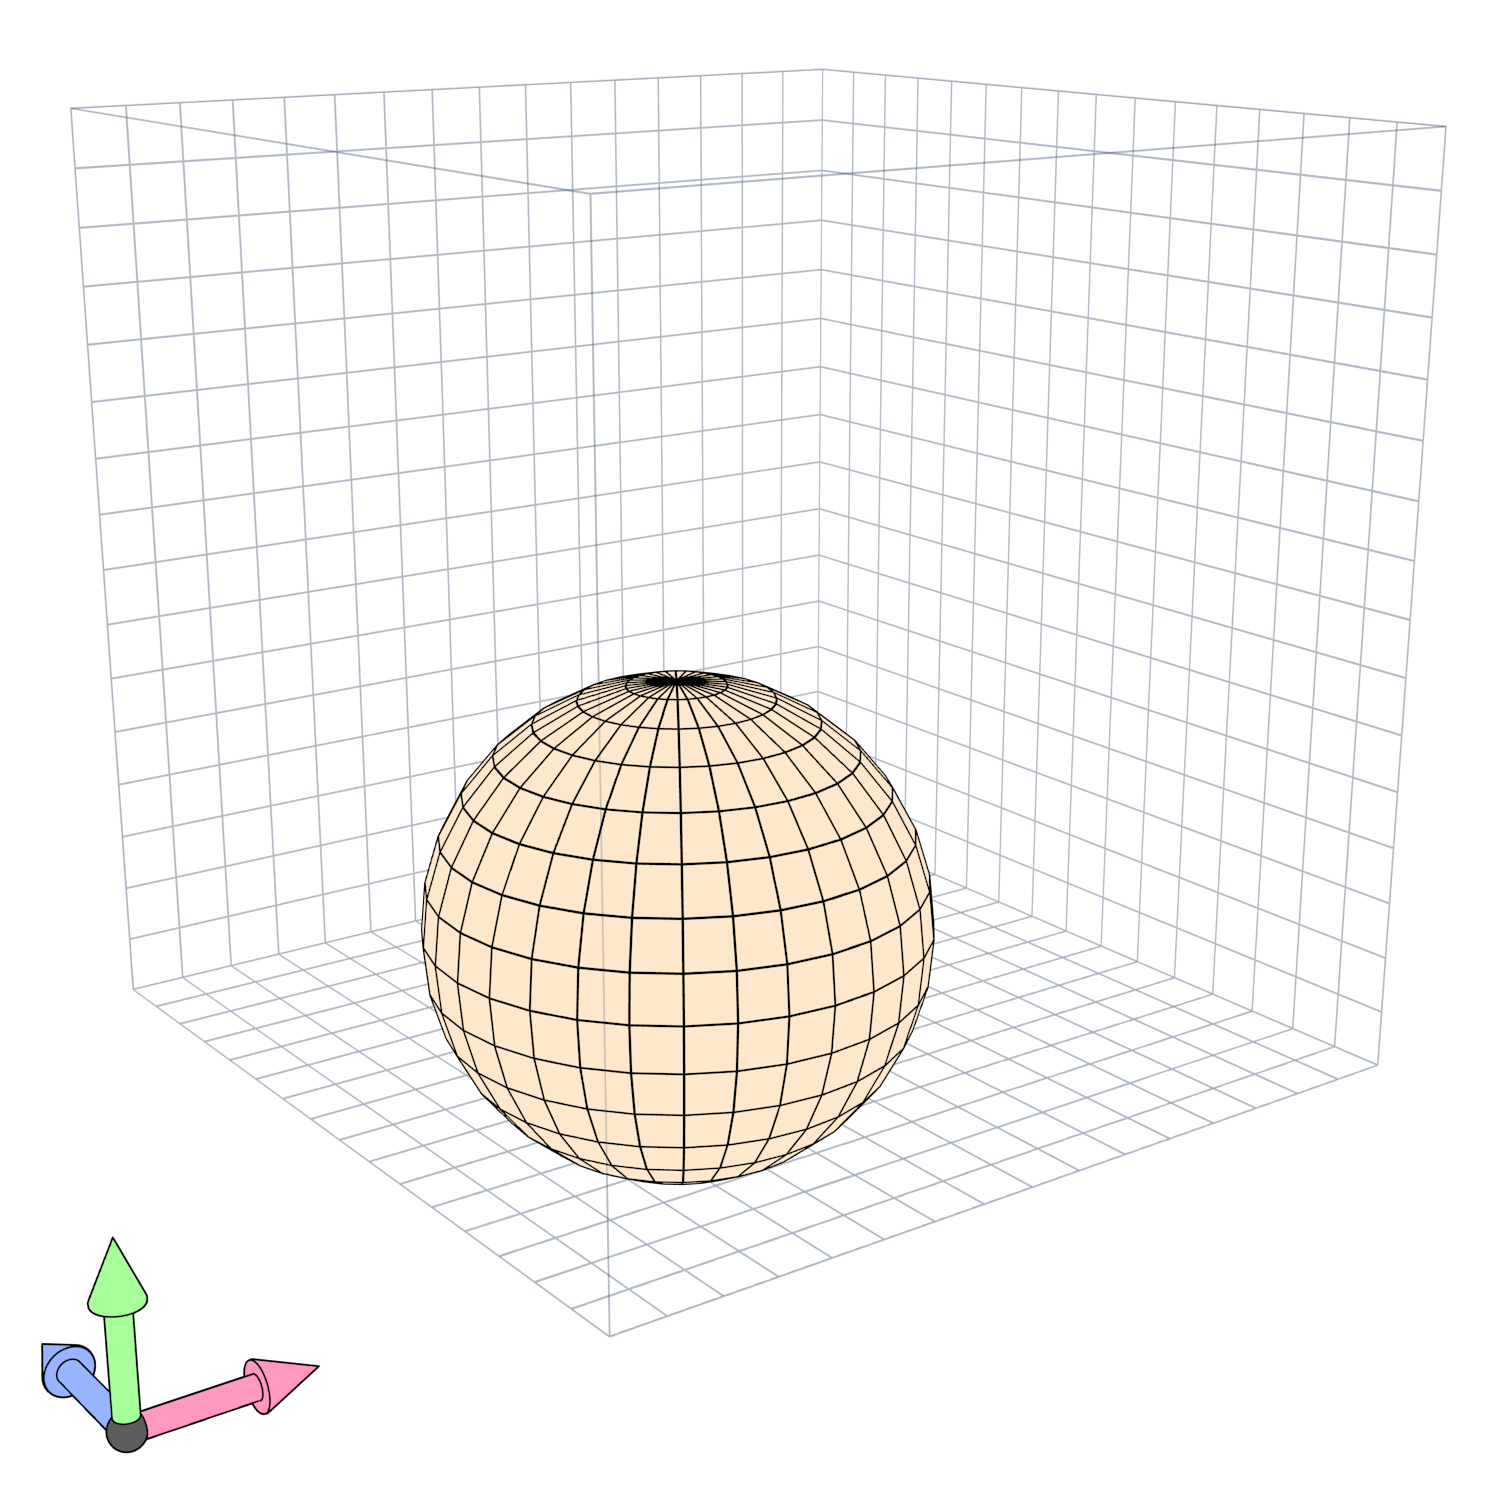
\includegraphics[width=\textwidth]{./img/raw/hs-slt/hs-slt_left.png}%
    \caption{Light volume}%
    \label{fig:hs-slt-left}%
  \end{subfigure} %
  \begin{subfigure}[b]{.45\linewidth}%
    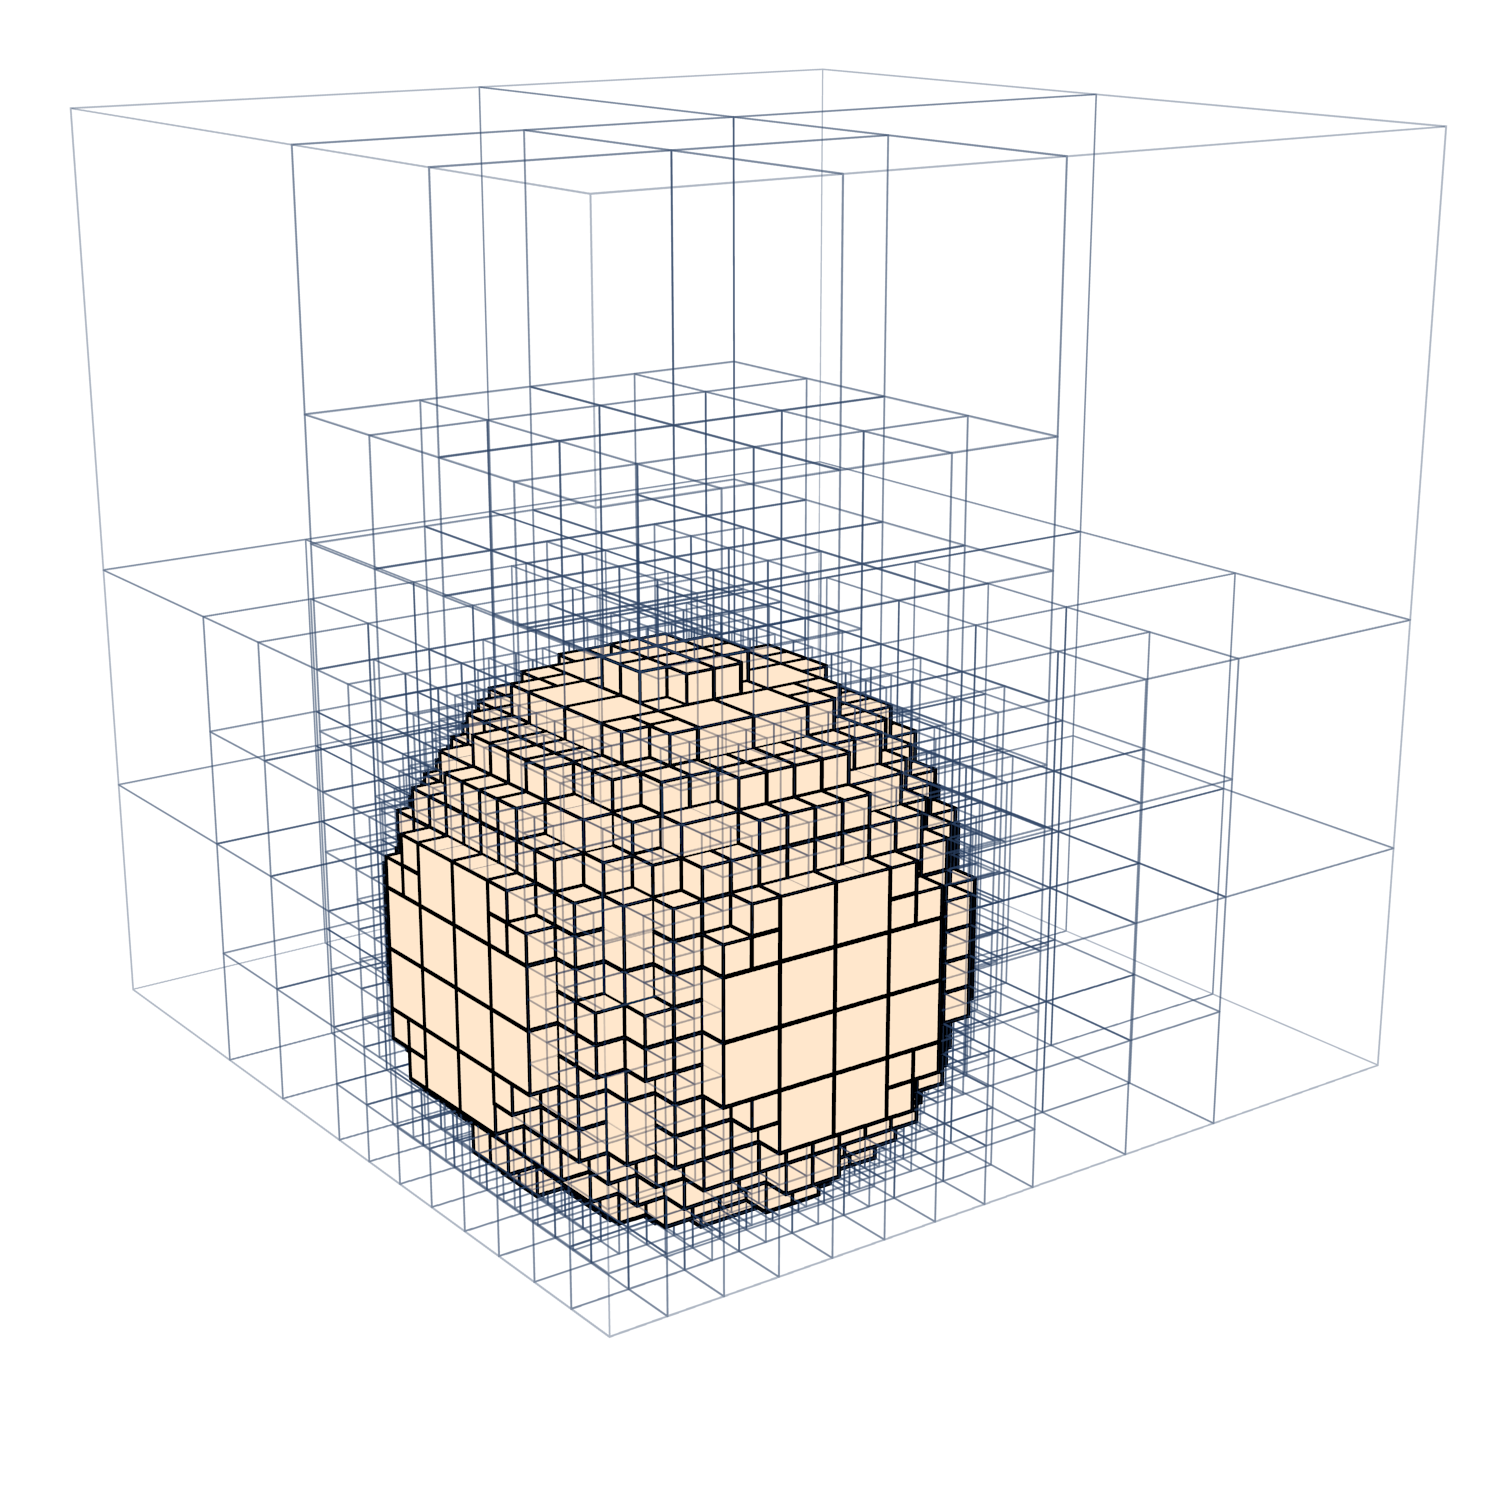
\includegraphics[width=\textwidth]{./img/raw/hs-slt/hs-slt_right.png}%
    \caption{Octree subdivision}%
    \label{fig:hs-slt-right}%
  \end{subfigure}
  \caption{Octree representation of a single light volume.}
  \label{fig:hs-slt}
\end{figure}


Finally the way these lights are represented in memory needs to be considered. If a light is
static during a whole simulation, there is no need to save the explicit influence of the
light separately and the overlapping nodes can all be combined in the scene octree.
However when a light is dynamic, the changing influence of the light on the subdivision of
the scene space needs to be calculated. This can be done efficiently by comparing the nodes
a light influences in the previous and current frame. Thus it is necessary to efficiently
represent each dynamic light in memory, in order to save computation time.
When the lights are small, or the node size is large, the grid could be saved directly in
memory. However when the node size is small compared to the point light radius, this leads
to unnecessary memory usage. The grid can be represented more compact by converting it into
an octree as well. This can be done in a top-down fashion by making use of the grid.
First the octree node which fully contains the grid is calculated. This node will serve
as a root node. For each node there are initially three possible options. The grid
does not overlap with the node, in which case the node is empty, as no overlapping nodes
lay outside of the grid. The grid partially overlaps with the node and the node falls
within the grid.

When the node overlaps partially there are two possibilities. Either the grid node
in the octree node closest to the light origin is overlapping, or it is not.
If it is, then the octree node is a branch node, and the eight children are evaluated.
If the grid node does not overlap with the light volume, the octree node is empty
as well.

In the last case there are three possibilities. If the grid node within the octree
node volume closest to the light origin is empty, the octree node will be empty
as well. If the closest grid node overlaps with the light volume, then either
the grid node within the octree node volume furthest from the light origin overlaps
with the light volume or it does not. In case it overlaps as well, then the whole
octree node volume overlaps, and thus the octree node is an overlapping leaf node.
If the furthest grid node does not overlap, the octree node contains both overlapping
and non-overlapping nodes, and the octree node is a branch node. The children of
this octree node are subsequently evaluated.

\subsection{Construction of the Scene Octree}

The scene octree is an octree structure of which the leaf nodes contain references
to the lights which overlap with the leaf node volumes. Depending on the representation
of the single lights, the scene octree can be constructed either top-down or bottom-up.

In case the lights are represented by the grid nodes which overlap with the light volume,
the nodes need to be combined first. This creates a set of nodes of minimum size that contain a set of
references to lights that overlap with these nodes. These can then be used to construct
the octree bottom-up. If the eight sibling nodes are leaf nodes and contain the same set of indices, it can
be replaced by a single leaf node in a higher layer, else a branch node in the layer above can be
added.

In case an octree representation is used, the scene octree can be build top-down by
recursively adding the light octrees to the scene octree. For each light octree the
scene octree node corresponding with the root of the light octree is found. Then the nodes
of the light octree are recursively added, where the filled light octree nodes are added
by adding the corresponding light index to the scene octree leaf node.

\subsection{Construction of the Linkless Octree and Light Index List}

As described in the overview, the octree nodes will specify a subset of the light index list.
Because this data is only saved in the leaf nodes of the scene octree. We opted for the
linkless octree variant that saves the data of the octree nodes separately from the octree
structure. Thus per layer a maximum of two spatial hash functions is constructed.

In the first step of construction of the linkless octree and light index list, the scene
octree nodes at the specified starting depth are gathered. For each of these nodes the
octree structure value is calculated as is specified in the algorithm of the linkless octree.
For each node we save whether the node is a leaf node, and whether the node contains any
information. If a node contains information, this information is stored in the second
spatial hash function. For each non-empty leaf node, the length of light index list
is saved, then the indices associated with the leaf node are added to the light index list.
The value saved in the second spatial hash function specifies the offset, equal to the length
of the light index list before adding the indices, and the length of the set of light indices.

\subsection{Light Assignment during Shading}

The final step of the algorithm is to use the constructed data structures to determine the set
of relevant lights per sample during the shading step. This step is similar to the shading
step of both Tiled and Clustered Shading. In order to find the subset of indices within the
light index list for a sample, we need to descend into the octree. For each layer we
calculate the octree structure of the node in which the sample falls. If this is a branch node,
the next layer is calculated. If the scene octree node is an empty leaf node, a vector containing
two zeroes is returned. If the the scene octree node is non-empty, the corresponding value is
obtained from the second spatial hash function of the current layer. The found offset and length
are returned.

Once the offset and length are obtained, the algorithm loops over the light indices within
the light index list, and for each light calculates the light contribution to the sample.
These values are summed and saved for the particular sample.


\section{Implementation}

In order to evaluate the Hashed Shading algorithm a new program, \texttt{nTiled},
was developed. This program was build with \texttt{C++} and \texttt{openGL} and
compiled with Visual Studio 2015. 
Besides the Hashed Shading algorithm, also a naive implementation which evaluates each
light per sample, and the Tiled and Clustered Shading algorithms were implemented.
All programs execute the same shading code, a simple white Lambertian material.

\subsection{Deferred Shading}

Deferred Shading is implemented by executing two render passes. In the first pass
the normal, a white albedo colour, and the depth are written to a GBuffer containing
the corresponding textures. In the second pass a full screen quad is rendered, and for
each generated sample the shading information is retrieved from the GBuffer and the
light contributions calculated.

\subsection{Tiled Shading}

In the forward and deferred Tiled shaders, the tiles which are influenced
by a light are determined by computing the bounding box of the projected light volume
in screen space\cite{mara20122d}. Then to each of the tiles overlapping with this
boundary box, the light index is added. This is all done on the CPU. The implementation
does not take into account the minimum and maximum $z$-values within tiles. Thus the
subdivision is not constrained with regards to these values.

\subsection{Clustered Shading}

Clustered Shading was implemented without the bounding volume hierarchy to assign
lights to the clusters specified in the original algorithm. The lights instead were
assigned in a brute force fashion by adjusting the Tiled Shading algorithm, and evaluating
whether it overlapped with any clusters which contained geometry. The sort and compact
step were implemented with \texttt{openGL} compute shaders. The assignment of lights is
implemented on the CPU which required the use of
\texttt{glGetTexImage}\footnote{\texttt{glGetTexImage}: {\tiny\url{https://www.khronos.org/registry/OpenGL-Refpages/gl4/html/glGetTexImage.xhtml}}}
This leads to a significant slowdown of the algorithm which skews the execution time results.

\subsection{Hashed Shading}

Hashed Shading is completely implemented on the CPU.  The individual lights are
represented by by octrees. The size of the offset hash table $\Phi$ is selected
by using the $\frac{n}{6}$ approximation, and increased geometrically until a correct
perfect spatial hash function is constructed. The offset and length values are
represented by 32 bit unsigned integers.

\section{Evaluation}

The performance of the Hashed Shading algorithm is evaluated with regards to both
the construction of the data structures and the execution during shading. The construction of
the data structures is evaluated with regards to both the time required to construct the
data structures as the memory they take up. The total amount of pixels required by the linkless
octree and the size of the Light Index List are used as indicators for this memory usage.

The performance of the shading is evaluated by timing the execution time per frame and by
calculating the total number of light calculations required to shade a frame in the
deferred pipeline. These values are compared to those of the Tiled and Clustered implementation.
Due to the performance issues of the Clustered Shading implementation the execution time of
Clustered Shading is not taken into account.

All timings are performed with the \texttt{QueryPerformanceCounter} provided on the Windows
platform.

The different tests were performed for three scenes:

\begin{itemize}
  \item Spaceship Indoor: an indoor spaceship scene based on CG Lighting Challenge \#18\footnote{scene url:\url{http://www.3drender.com/challenges/}}.
  \item Piper's Alley: a street scene based on CG Lighting Challenge \#42\footnote{scene url:\url{http://forums.cgsociety.org/archive/index.php?t-1309021.html}}.
  \item Ziggurat City: A shot from the open movie Sintel\footnote{open movie url: \url{durian.blender.org}}.
\end{itemize}

\noindent These scenes were chosen to represent the different potential game environments.


% Add information about how the nodde sizes are related
% Latter compared to Tiled and Clustered Shading

% Construction Time and Memory Usage
% The performance of Hashed Shading algorithm is evaluated with regards to both its construction
% and the execution. For the construction the construction time is evaluated. Furthermore the
% number of pixels used in the perfect spatial hash functions and the size of the light index
% list are evaluated.

% Light calculations and execution time
% The execution time of both the Forward and the Deferred Pipeline are compared to the Tiled and
% naive implementations. Due to complications with the Clustered Shading implementation, its
% execution time is not taken into account. The number of light calculations per frame for
% the deferred naive implementation, deferred tiled shading, deferred clustered shading and
% deferred hashed shading were also compared.

% 3 scenes used
% All tests were done for three scenes. An indoor spaceship scene was based on CG Lighting
% Challenge \#18\footnote{}. A street scene was based on CG Lighting Challenge \#42\footnote{}.
% And a city scene based on a scene from the open movie Sintel\footnote{}. These scenes were
% chosen to represent different possible game environments. For each scene light generation
% volumes were defined. Within these volumes different number of lights were generated, to
% create different number of lights for each scene.

The influence of both the number of lights, as the resolution on the execution time and
number of lights of the different light assignment algorithms is evaluated. For this six
different resolutions ranging from $320 \times 320$ to $2560 \times 2560$ are evaluated, and
number of lights ranging from less than a hundred till more than a thousand lights per
scene are evaluated.

All of these simulations were executed on a Dell XPS laptop with the following hardware:

\begin{table}[h!]
  \begin{tabular}{@{}ll@{}}\toprule
    Operating system       & Windows 10 64-bit                \\
    CPU & Inter Core i7 6700 HQ @ 2.60 Ghz \\
    Memory & 16 GB                            \\
    GPU & NVIDIA GeForce GTX 960M          \\
    GPU drivers & 372.70                           \\ \bottomrule
  \end{tabular}
\end{table}


\section{Results and Discussion}

In order for Hashed Shading to be viable its performance needs to be at least on par
with Tiled and Clustered Shading. This requires a low memory footprint and a similar
reduction in execution time and number of light calculations.

% In order for Hashed Shading to be viable, it would need to perform similarly to
% Tiled and Clustered Shading. Furthermore it should not use an excessive amount
% of memory. 


\subsection{Construction Time and Memory Usage}

The results of the construction time as function of the node size relative to the radius
of the lights for different number of lights can be found in
figure \ref{fig:hs-ns-construction-time}. The construction time for individual functions
for the largest sets of lights can be found in figure \ref{fig:hs-layered-exec}. A cubic
relationship between the node size and the construction time can be
clearly observed. This leads to a  significant increase of construction time when more
than $8^3$ nodes are required to contain a light volume.
This increase in construction time is primarily due to the construction of the spatial
hash functions representing the layers of the linkless octree.

The same cubic relationship can be seen between the memory usage and the node size. Both the
combined number  of pixels used in the spatial hash functions of the linkless octree,
fig \ref{fig:hs-ns-memory}, and the size of the Light Index List, fig \ref{fig:hs-ns-light-indices},
show cubic growth with regards to a smaller node size. Figure \ref{fig:hs-layered-mem:octree}
and \ref{fig:hs-layered-mem:data} show that
the majority of the pixels used in the linkless octree
are used within the deepest layers of the linkless octree. This indicates that
a significant number of leaf nodes exist in the deepest layers of the linkless octree,
when the node size decreases. This is further supported by the increase in size of the Light
Index List. Each leaf node adds its set of light indices to the Light Index List. Thus the
total size of the Light Index List is an indicator for the total number of leaf nodes.
A smaller node size allows for a more fine-grained description of scene space. When lights
partially overlap the leaf nodes can not be combined as their light index sets differ. A
smaller node size will increase this effect, and more small octree nodes will be spawned
as a result.

The node size effects the size in all three dimensions of the node. Thus a reduction of the
node size potentially leads to a cubic increase in number of nodes. This cubic increase
of nodes is the source of the increase in number of nodes which drives up the memory usage
and construction time.

The influence of the starting depth on the construction time and the combined size of the textures
is shown in figure \ref{fig:hs-sd-construction} and \ref{fig:hs-sd-memory} respectively.
The construction time and memory usage
are not effected by this change. However, the memory overhead is reduced as
the total number of required textures is reduced. Increasing the starting depth
removes the shallowest layers of the linkless octree. These have a relatively small
influence on the total memory usage and the construction time as the spatial hash functions
are small compared to the deeper layers of the linkless octree. Thus a greater starting depth
can be used to reduce the overhead of the textures and the total number of textures used,
without significantly increasing the amount of nodes required. Furthermore
removing the shallowest layers of the octree will reduce the number of memory accesses
during the shading step, thus improving the performance during shading.

% The results of the construction time for different number of lights as function of the
% node size can be found in figure \ref{}. The construction time of the individual steps
% are shown in figure \ref{}. We can clearly see a cubic relation between the node size
% and the execution time. This leads to a significant increase when more than $8^3$ nodes per
% light are used. This is primarily due to the construction time of the spatial hash functions
% which represent the layers.

% The same cubic relationship can be seen in the memory usage. Both the size of the light index
% list and the combined number of pixels within the textures used by the linkless octree show
% cubic growth with regards to a smaller node size. The majority of the memory is used in
% the deepest layers of the linkless octree. The size of the light index list is an indication
% for the number of non-empty leaf nodes. A smaller node size allows for a more fine grained
% representation of space, thus, partly overlapping lights will produce more deep octree nodes.
% The overlap within lights will create a difference in the light set contained in the nodes,
% and thus spawn a larger number of small octree nodes.

% The node size affects the size in all three dimensions of the node, thus if the node size
% is halved it will span $\frac{1}{2}^3 = 8$ times as many nodes. This cubic increase in
% nodes drives both the memory usage, and the construction time.

\subsection{Execution Time and Light Calculations}

Figure \ref{fig:hs-compare-frames:forward} and \ref{fig:hs-compare-frames:deferred} show the
execution time per frame for the forward and deferred pipelines
during a single simulation of both Tiled and Hashed Shading. Figure \ref{fig:hs-compare-frames:lc}
shows the number of light calculations per frame during a single simulation of the deferred pipeline for
Tiled, Clustered and Hashed Shading.

In the deferred pipeline a similar performance with regards to the execution time can be observed for
both Tiled and Hashed Shading, even though the Hashed Shading implementation requires only
half of the light calculations. This is a result of the simplicity of the used fragment shader.
The bottleneck in this case is not the shading pass but the geometry pass. The change in number
of calculations does not influence the geometry pass, thus performance is comparable. When
the complexity of the shader, and therefore the amount of work during the shading pass, is
increased the difference in the number of light calculations should become noticeable.
The Forward Hashed Shading implementation does perform about twice as well as the Forward
Tiled Shading implementation, which is in line with the reduction of the number of light
calculations achieved with Hashed Shading. The forward pipeline has significant overdraw,
thus per pixel multiple fragments are evaluated. This amplifies the influence of the
reduction of the number of light calculations.

For small node size the reduction of light calculations achieved by Hashed Shading approaches
that of Clustered Shading. When the node size would be reduced further, it should equate
and potentially surpass Clustered Shading.

% Figure \ref{} shows the execution time for both the forward and deferred pipelines during
% a single evaluation of both hashed shading and tiled shading. Figure \ref{} shows the
% number of light calculations during a single simulation of the deferred pipeline for
% tiled, clustered and hashed shading.

% In the Deferred Pipeline we can see a similar performance for Tiled and Hashed Shading.
% However Hashed Shading requires a factor two less light calculations. Due to the simple
% fragment shader used, this difference in number of light calculations is not significant
% enough to create a difference in execution time. If a more complex shader would be used,
% the difference in number of light calculations should be noticeable. The Forward Shading
% pipeline has a significant amount of overdraw, thus a larger number of fragments per
% pixel is evaluated. In this situation Hashed Shading performs about two times faster,
% in line with the results from the reduction in number of light calculations.

% For small node sizes the Hashed Shading algorithm approaches the reduction in light calculations
% of Clustered Shading. While Clustered Shading still requires less light calculations, the
% difference in minimal. A further reduction in node size should reduce the gap in light calculations.

In figure \ref{fig:hs-compare-lights:forward} and \ref{fig:hs-compare-lights:deferred} the average
execution time per frame for the Forward and Deferred pipelines as
function of the number of lights is plotted. All of the algorithms scale linearly with the
number of lights. The results are comparable to those observed for the single simulation. For Deferred
Shading the performance increase of Hashed Shading is similar to that of Tiled Shading. In
the Forward pipeline, again an improvement of a factor two is noticeable.
The number of light calculations, figure \ref{fig:hs-compare-lights:lc}, shows that the
reduction in calculation time is a direct result of the reduction of number of light calculations.
The smallest node size shows a comparable curve to that of Clustered Shading.

The behaviour with regards to the resolution is shown in figure \ref{fig:hs-compare-resolution:forward},
\ref{fig:hs-compare-resolution:deferred} and \ref{fig:hs-compare-resolution:lc}.
Both the execution time and the number of light calculations are linearly dependent on
the number of fragments. 
Hashed Shading performs slightly better with increasing resolutions, though the effect
is almost negligible. The memory usage of both Tiled and Clustered Shading is directly
linked to the size of view port. Hashed Shading has no such dependency, thus it will not
be significantly affected by changing resolutions. With the trend of growing resolutions,
this might prove to be an important attribute of Hashed Shading.


\section{Conclusion}

In this paper the Hashed Shading algorithm has been presented and evaluated. Hashed Shading is
a light assignment algorithm which subdivides the scene space independently of the
view frustum. This subdivision is then stored in a linkless octree which can be queried during
shading. Because the subdivision is independent of the view frustum, changes in the camera
position and orientation do not require a complete recalculation of the data structures. Thus the
data structures can be reused between frames.

The Hashed Shading algorithm performs better than the Tiled Shading algorithm and
approaches the reduction of light calculations achieved by Clustered Shading.
Furthermore Hashed Shading performs slightly better with increasing resolutions
compared to both Tiled and Clustered Shading, because its subdivision does not
depend directly on the direction.

However there are still two major problems with the current Hashed Shading implementation.
The memory footprint increases cubicly with a decreasing node size. This leads
to unacceptable memory requirements for small node sizes. Secondly dynamic lights
are not currently not supported within the Hashed Shading implementation. Adding
this support would increase computation time during shading.

Overall it can be concluded that camera-independent light assignment is a viable strategy.
The decoupling of resolution could play a role with the trend of increasing screen resolutions.
Future work would need to solve the memory requirements and allow for efficient support
of dynamic lights in order for Hashed Shading and similar algorithms to be competitive with
Clustered Shading.

% In this paper we have presented and evaluated the Hashed Shading algorithm. In Hashed Shading
% the scene space is divided independent of the camera with a linkless octree data structure.
% The linkless octree allows for efficient light assignment and reuse of data structures between
% frames. We have shown that it is possible to achieve better performance than Tiled Shading
% by using this camera-independent data structure. Furthermore for small node sizes, the
% number of light calculations approaches that of Clustered Shading, and could potentially
% exceed it. There are two problems with the current implementation of Hashed Shading;
% no dynamic lights are supported and the memory footprint is large. These two issues need
% to be addressed before Hashed Shading becomes a viable alternative for Tiled and Clustered
% Shading.

\section{Future work}

The two main issues with the current implementation of Hashed Shading are the large memory
footprint and the lack of support for dynamic lights. These two issues have to be addressed
before Hashed Shading can become a viable alternative to Clustered Shading. Proposals
to solve those two issues are introduced in the next sections.

Besides these two issues, there are several other directions for future work. Currently
the Hashed Shading implementation only supports point lights. In order to support
other light types, strategies to convert their light volumes into octrees need to be
drafted. The current implementation also does not support shadows currently. There
are several algorithms which leverage the clustered shading clusters to reduce
the amount of work required to support shadows within Clustered Shading\cite{Olsson:2014:EVS:2556700.2556701, kampe2016fast}.
Similar approaches could be used to support shadows in Hashed Shading by leveraging
the octree data structure.

% Besides these two issues there are several other options for future work. Currently
% the Hashed Shading algorithm only supports point lights, in order to support other
% lights, their volumes need to be represented as octrees efficiently. Secondly
% the current implementation has no support for shadows. There are several ways in which
% the Clustered Shading clusters are leveraged to reduce the work required to calculate
% shadows\cite{}. Similar techniques could be developed by using the Hashed Shading octree.

\subsection{Memory Usage Reduction}
\subsubsection{Geometry}

\begin{figure}[t]
  \centering
  \begin{subfigure}[b]{0.249\textwidth}
    \centering
  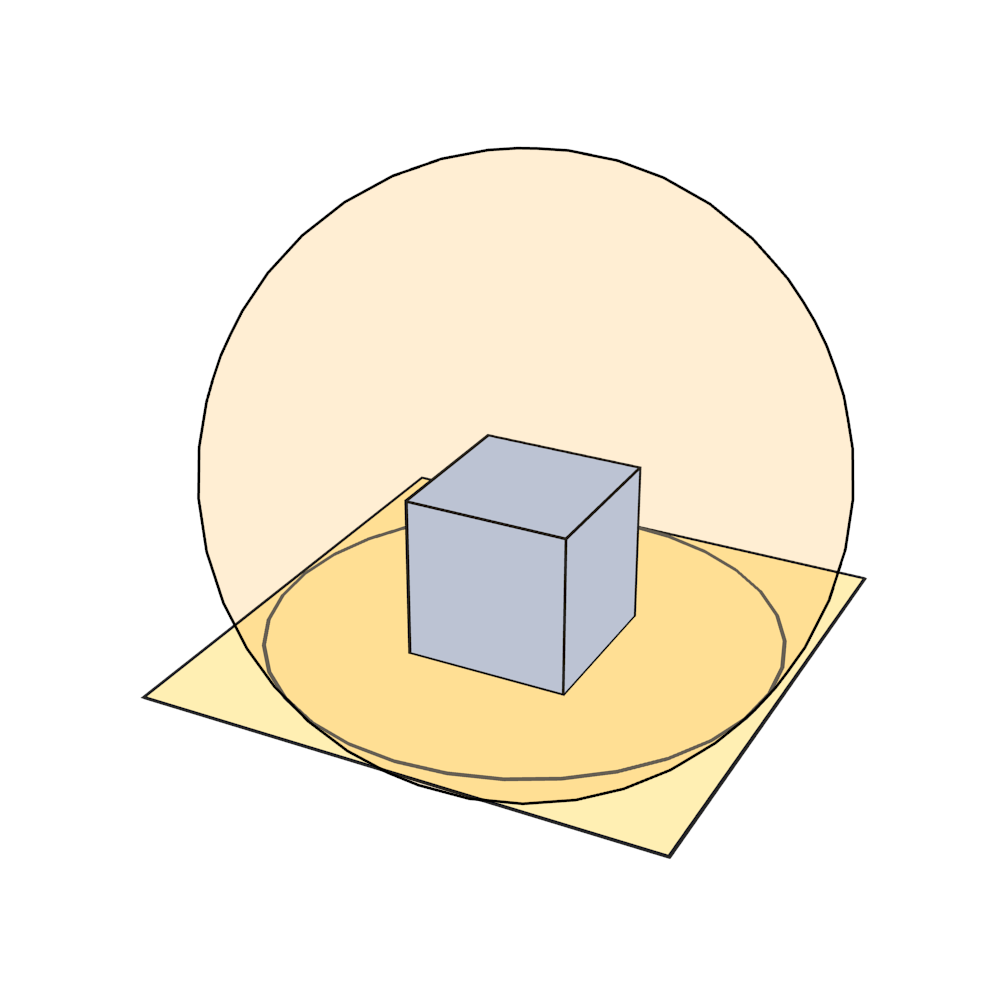
\includegraphics[width=\textwidth]{./img/raw/besluit-geom/scene.png}
  \caption{Simple scene.}
  \label{fig:vo-geometrie:0}
  \end{subfigure}%
  \begin{subfigure}[b]{0.249\textwidth}
    \centering
  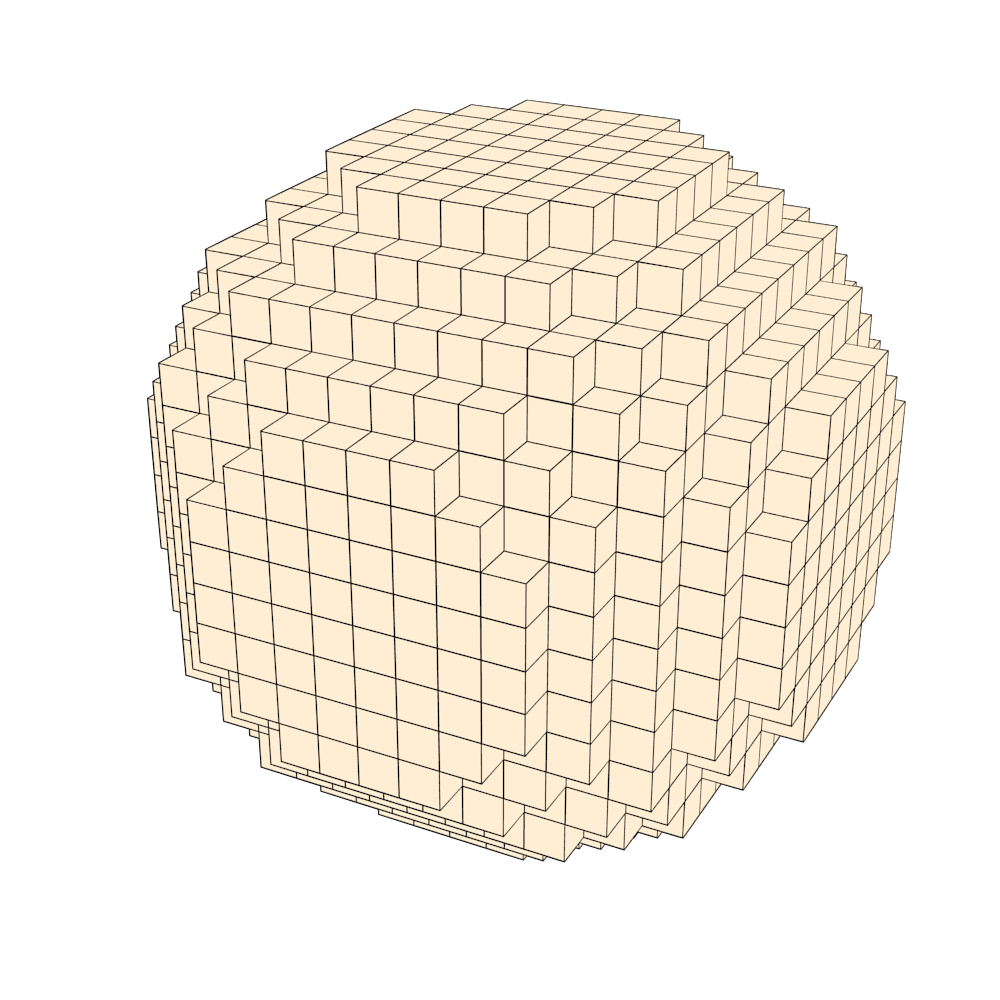
\includegraphics[width=\textwidth]{./img/raw/besluit-geom/light.png}
  \caption{Light nodes.}
  \label{fig:vo-subsets:1}
  \end{subfigure}\\
  \begin{subfigure}[b]{0.249\textwidth}
    \centering
  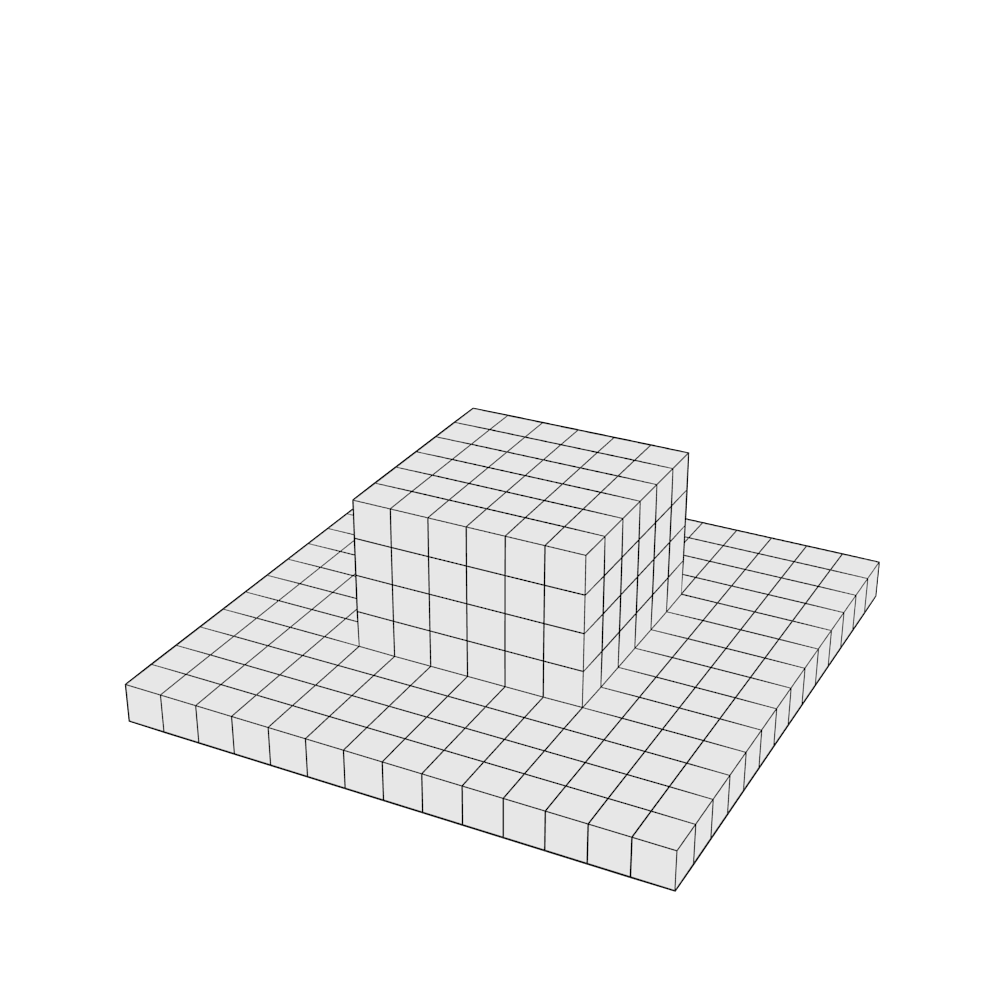
\includegraphics[width=\textwidth]{./img/raw/besluit-geom/geom.png}
  \caption{Geometry nodes.}
  \label{fig:vo-geometrie:0}
  \end{subfigure}%
  \begin{subfigure}[b]{0.249\textwidth}
    \centering
  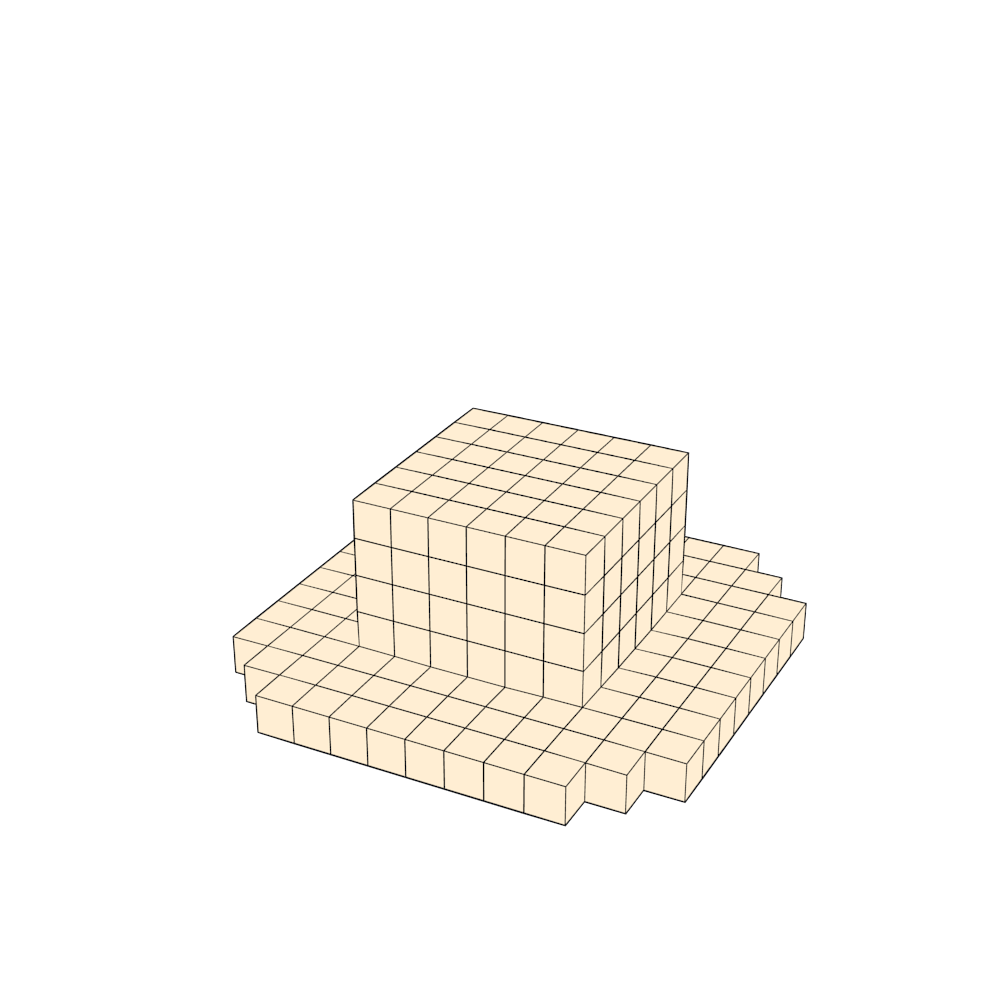
\includegraphics[width=\textwidth]{./img/raw/besluit-geom/comb.png}
  \caption{Light geometry nodes.}
  \label{fig:vo-subsets:1}
  \end{subfigure}
  \caption{Reduction of the number of nodes by excluding empty space.}
  \label{fig:vo-geometrie}
\end{figure}


An important insight Clustered Shading leverages to reduce the memory usage is that samples
will only be generated in clusters that contain geometry. Thus there is no need to construct
clusters that will not generate samples. A similar approach can be used in Hashed Shading.
A second octree with the same size and origin can be constructed for the geometry, where in
the leaf node is stored if the corresponding volume contains geometry. This octree can then
be used to determine whether a node has to be saved or not. Only if a node contains geometry
it needs to be physically saved, and only if the node contains both lights and geometry it
needs to be saved in the second spatial hash function. Thus such an octree could greatly
reduce the number of nodes as is shown in figure \ref{fig:vo-geometrie}.

A second advantage of this approach would be that a smaller node size would not directly
cubicly increase the number of nodes. As a smaller node size would also increase the
precision with which the geometry is represented, it would actually increase the amount of
empty space, thus reducing the amount of nodes that need to be kept in memory.

Lastly the conditions required for a set of sibling nodes to be combined into a single
parent node could be weakened. Since nodes which do not contain any geometry data will
never be queried, an arbitrary value could be assigned to them, without influencing the
performance of Hashed Shading. The current condition requires all the sibling nodes to
have the same set of lights, before they can be combined into a single leaf node. With
this optimalisation this can be reduced to all sibling nodes which contain geometry
need to contain the same set of lights. This would further reduce the number of nodes
needed to represent the scene space.

\subsubsection{Subdivision of Space}

\begin{figure}
  \usetikzlibrary{shapes.arrows, positioning}
  \definecolor{LightColor}{rgb}{1.0,0.901,0.805}
  \definecolor{EmptyColor}{HTML}{DCE2E6}

  \definecolor{tile0}{HTML}{DABDE4}
  \definecolor{tile1}{HTML}{B8DBF4}
  \definecolor{tile2}{HTML}{B5EDCD}
  \definecolor{tile3}{HTML}{FBEBA7}
  \definecolor{tile4}{HTML}{F9C1BB}
  \definecolor{tile5}{rgb}{1, 1, 1}

  \tikzstyle{array_element}=[rectangle,
                             minimum height=0.5cm, 
                             minimum width=0.5cm, 
                             minimum size=0.5cm,
                             draw=black,
                             rounded corners=2.5, ]
  \tikzstyle{empty_element}=[rectangle,
  fill=white
                                ]


  \begin{adjustbox}{minipage=\textwidth, scale=0.425}
    \centering
\begin{tikzpicture}
     \node at (0.5cm * 0 + 0.1cm * 0, 0) (H) [array_element, fill=LightColor] {};
     \node at (0.5cm * 1 + 0.1cm * 1, 0) (H) [array_element, fill=tile2] {};

     \node at (0.5cm * 1 + 0.1cm * 1 + 1.5cm * 1, 0) (H) [array_element, fill=LightColor] {};
     \node at (0.5cm * 2 + 0.1cm * 1 + 1.5cm * 1, 0) (H) [array_element, fill=LightColor] {};
     \node at (0.5cm * 1 + 0.1cm * 1 + 1.5cm * 1, -0.5cm) (H) [array_element, fill=LightColor] {};
     \node at (0.5cm * 2 + 0.1cm * 1 + 1.5cm * 1, -0.5cm) (H) [array_element, fill=LightColor] {};
     
     \node at (0.5cm * 3 + 0.1cm * 2 + 1.5cm * 1, -0.0cm) (H) [array_element, fill=tile2] {};

    \node at (0.5cm * 1 + 0.1cm * 1 + 0.25cm, -0.cm) (c1) [] {};
    \node at (0.5cm * 1 + 0.1cm * 1 + 1.5cm * 1 - 0.25cm, -0.cm) (c2) [] {};
    \draw[-latex](c1) -- (c2);

    \node at (0.5cm * 3 + 0.1cm * 2 + 1.5cm * 1 + 0.25cm, -0.cm) (c1) [] {};
    \node at (0.5cm * 3 + 0.1cm * 2 + 1.5cm * 1 + 2.5cm - 0.25cm, -0.cm) (c2) [] {};
    \draw[-latex](c1) --node[empty_element, pos=0.525] {$\dots$} (c2);

    \node at (0.5cm * 8 + 0.1cm * 3 + 1.5cm * 1 + 2.5cm + 0.25cm, -0.cm) (c1) [] {};
    \node at (0.5cm * 8 + 0.1cm * 3 + 1.5cm * 2 + 2.5cm - 0.25cm, -0.cm) (c2) [] {};
    \draw[-latex](c1) -- (c2);

    \node at (0.5cm * 16 + 0.1cm * 4 + 1.5cm * 1 + 2.5cm + 0.25cm, -0.cm) (c1) [] {};
    \node at (0.5cm * 16 + 0.1cm * 4 + 1.5cm * 2 + 2.5cm - 0.25cm, -0.cm) (c2) [] {};
    \draw[-](c1) --node[empty_element, pos=1] {$\dots$} (c2);



    \foreach \la in {0,...,3} {
        \foreach \lb in {0,...,3} {
            \node at (0.5cm * \la + 0.5cm * 3 + 0.1cm * 2 + 1.5cm * 1 + 2.5cm, -0.5cm * \lb) (H\la\lb) [array_element, fill=LightColor] {};
        }
    }
    \foreach \la in {0,...,1} {
        \foreach \lb in {0,...,1} {
            \node at (0.5cm * \la + 0.5cm * 7 + 0.1cm * 3 + 1.5cm * 1 + 2.5cm , -0.5cm * \lb) (H\la\lb) [array_element, fill=tile2] {};
        }
    }

    \foreach \la in {0,...,3} {
        \foreach \lb in {0,...,3} {
            \node at (0.5cm * \la + 0.5cm * 8 + 0.1cm * 3 + 1.5cm * 2 + 2.5cm, -0.5cm * \lb) (H\la\lb) [array_element, fill=LightColor] {};
        }
    }
    \foreach \la in {0,...,1} {
        \foreach \lb in {0,...,1} {
            \node at (0.5cm * \la + 0.5cm * 12 + 0.1cm * 4 + 1.5cm * 2 + 2.5cm , -0.5cm * \lb) (H\la\lb) [array_element, fill=tile2] {};
        }
    }



      \foreach \la in {0,...,3} {
        \node at (0.5cm * 2 + 0.1cm * 1 + 1.0cm, -3cm - 1.25cm * \la) (H) [array_element, fill=LightColor] {};
        \node at (0.5cm * 3 + 0.1cm * 2 + 1.0cm, -3cm - 1.25cm * \la) (H) [array_element, fill=tile2] {};
        
             \node at (0.5cm * 0 + 0.1cm * 2 + 1.5cm * 2 + 2.5cm, -3cm -1.25cm * \la) (H) [array_element, fill=LightColor] {};
     \node at (0.5cm * 1 + 0.1cm * 2 + 1.5cm * 2  + 2.5cm, -3cm -1.25cm * \la) (H) [array_element, fill=LightColor] {};
     \node at (0.5cm * 0 + 0.1cm * 2 + 1.5cm * 2 + 2.5cm, -0.5cm -3cm -1.25cm * \la) (H) [array_element, fill=LightColor] {};
     \node at (0.5cm * 1 + 0.1cm * 2 + 1.5cm * 2 + 2.5cm, -0.5cm - 3cm -1.25cm * \la) (H) [array_element, fill=LightColor] {};
     \node at (0.5cm * 2 + 0.1cm * 3 + 1.5cm * 2 + 2.5cm, -0.0cm - 3cm -1.25cm * \la) (H) [array_element, fill=tile2] {};
     
         \node at (0.5cm * 2 + 0.1cm * 2 + 1.5cm * 1 + 0.25cm, -0.cm - 3cm -1.25cm * \la) (c1) [] {};
    \node at (0.5cm * 3 + 0.1cm * 2 + 1.5cm * 1 + 2.5cm - 0.25cm, -0.0cm - 3cm -1.25cm * \la) (c2) [] {};
    \draw[-latex](c1) --node[empty_element, pos=0.525] {$\dots$} (c2);

     \node at (0.5cm * 6 + 0.1cm * 3 + 1.5cm * 3 + 2.5cm, -3cm -1.25cm * \la) (H) [array_element, fill=LightColor] {};
     \node at (0.5cm * 5 + 0.1cm * 3 + 1.5cm * 3  + 2.5cm, -3cm -1.25cm * \la) (H) [array_element, fill=LightColor] {};
     \node at (0.5cm * 5 + 0.1cm * 3 + 1.5cm * 3 + 2.5cm, -0.5cm -3cm -1.25cm * \la) (H) [array_element, fill=LightColor] {};
     \node at (0.5cm * 6 + 0.1cm * 3 + 1.5cm * 3 + 2.5cm, -0.5cm - 3cm -1.25cm * \la) (H) [array_element, fill=LightColor] {};
     \node at (0.5cm * 7 + 0.1cm * 4 + 1.5cm * 3 + 2.5cm, -0.0cm - 3cm -1.25cm * \la) (H) [array_element, fill=tile2] {};

    \node at (0.5cm * 2 + 0.1cm * 4 + 1.5cm * 2 + 2.5cm + 0.25cm, -0.cm -3cm -1.25cm * \la) (c1) [] {};
    \node at (0.5cm * 5 + 0.1cm * 3 + 1.5cm * 3 + 2.5cm - 0.25cm, -0.cm-3cm -1.25cm * \la) (c2) [] {};
    \draw[-latex](c1) -- (c2);

    \node at (0.5cm * 16 + 0.1cm * 4 + 1.5cm * 1 + 2.5cm + 0.25cm - 1.5cm, -3cm -1.25cm * \la) (c1) [] {};
    \node at (0.5cm * 16 + 0.1cm * 4 + 1.5cm * 2 + 2.5cm - 0.25cm - 1cm, -3cm -1.25cm * \la) (c2) [] {};
    \draw[-](c1) --node[empty_element, pos=1] {$\dots$} (c2);
      }

     \node at (0.5cm * 0 + 0.1cm * 0, 0 - 8.75cm) (H) [array_element, fill=LightColor] {};
     \node at (0.5cm * 1 + 0.1cm * 1, 0- 8.75cm) (H) [array_element, fill=tile2] {};

     \node at (0.5cm * 1 + 0.1cm * 1 + 1.5cm * 1, 0- 8.75cm) (H) [array_element, fill=LightColor] {};
     \node at (0.5cm * 2 + 0.1cm * 1 + 1.5cm * 1, 0 - 8.75cm) (H) [array_element, fill=LightColor] {};
     \node at (0.5cm * 1 + 0.1cm * 1 + 1.5cm * 1, -0.5cm - 8.75cm) (H) [array_element, fill=LightColor] {};
     \node at (0.5cm * 2 + 0.1cm * 1 + 1.5cm * 1, -0.5cm - 8.75cm) (H) [array_element, fill=LightColor] {};
     
     \node at (0.5cm * 3 + 0.1cm * 2 + 1.5cm * 1, -0.0cm - 8.75cm) (H) [array_element, fill=tile2] {};

    \node at (0.5cm * 1 + 0.1cm * 1 + 0.25cm, -0.cm - 8.75cm) (c1) [] {};
    \node at (0.5cm * 1 + 0.1cm * 1 + 1.5cm * 1 - 0.25cm, -0.cm - 8.75cm) (c2) [] {};
    \draw[-latex](c1) -- (c2);

    \node at (0.5cm * 3 + 0.1cm * 2 + 1.5cm * 1 + 0.25cm, -0.cm - 8.75cm) (c1) [] {};
    \node at (0.5cm * 3 + 0.1cm * 2 + 1.5cm * 1 + 2.5cm - 0.25cm, -0.cm - 8.75cm) (c2) [] {};
    \draw[-latex](c1) --node[empty_element, pos=0.525] {$\dots$} (c2);

    \node at (0.5cm * 8 + 0.1cm * 3 + 1.5cm * 1 + 2.5cm + 0.25cm, -0.cm - 8.75cm) (c1) [] {};
    \node at (0.5cm * 8 + 0.1cm * 3 + 1.5cm * 2 + 2.5cm - 0.35cm, -0.cm - 8.75cm) (c2) [] {};
    \draw[-latex](c1) -- (c2);
    
        \node at (0.5cm * 8 + 0.1cm * 3 + 1.5cm * 1 + 2.5cm + 0.25cm, -0.cm - 8.75cm - 0.5cm) (c1) [] {};
    \node at (0.5cm * 8 + 0.1cm * 3 + 1.5cm * 2 + 2.5cm - 0.35cm, -0.cm - 8.75cm - 1.25 cm) (c2) [] {};
    \draw[-latex](c1) -- (c2);

        \node at (0.5cm * 8 + 0.1cm * 3 + 1.5cm * 1 + 2.5cm + 0.25cm, -0.cm - 8.75cm  - 0.5cm * 2) (c1) [] {};
    \node at (0.5cm * 8 + 0.1cm * 3 + 1.5cm * 2 + 2.5cm - 0.35cm, -0.cm - 8.75cm - 1.25 cm * 2) (c2) [] {};
    \draw[-latex](c1) -- (c2);

        \node at (0.5cm * 8 + 0.1cm * 3 + 1.5cm * 1 + 2.5cm + 0.25cm, -0.cm - 8.75cm - 0.5cm * 3) (c1) [] {};
    \node at (0.5cm * 8 + 0.1cm * 3 + 1.5cm * 2 + 2.5cm - 0.35cm, -0.cm - 8.75cm - 1.25 cm * 3) (c2) [] {};
    \draw[-latex](c1) -- (c2);


        \foreach \la in {0,...,3} {
        \foreach \lb in {0,...,3} {
            \node at (0.5cm * \la + 0.5cm * 3 + 0.1cm * 2 + 1.5cm * 1 + 2.5cm, -0.5cm * \lb - 8.75cm) (H\la\lb) [array_element, fill=LightColor] {};
        }
    }
    \foreach \la in {0,...,1} {
        \foreach \lb in {0,...,1} {
            \node at (0.5cm * \la + 0.5cm * 7 + 0.1cm * 3 + 1.5cm * 1 + 2.5cm , -0.5cm * \lb - 8.75cm) (H\la\lb) [array_element, fill=tile2] {};
        }
    }
    \foreach \la in {0,...,3} {
         \node at (0.5cm * 6 + 0.1cm * 3 + 1.5cm * 3 + 2.5cm, -3cm -1.25cm * \la - 5.75cm) (H) [array_element, fill=LightColor] {};
     \node at (0.5cm * 5 + 0.1cm * 3 + 1.5cm * 3  + 2.5cm, -3cm -1.25cm * \la - 5.75cm) (H) [array_element, fill=LightColor] {};
     \node at (0.5cm * 5 + 0.1cm * 3 + 1.5cm * 3 + 2.5cm, -0.5cm -3cm -1.25cm * \la - 5.75cm) (H) [array_element, fill=LightColor] {};
     \node at (0.5cm * 6 + 0.1cm * 3 + 1.5cm * 3 + 2.5cm, -0.5cm - 3cm -1.25cm * \la - 5.75cm) (H) [array_element, fill=LightColor] {};
     \node at (0.5cm * 7 + 0.1cm * 4 + 1.5cm * 3 + 2.5cm, -0.0cm - 3cm -1.25cm * \la - 5.75cm) (H) [array_element, fill=tile2] {};
    \node at (0.5cm * 16 + 0.1cm * 4 + 1.5cm * 1 + 2.5cm + 0.25cm - 1.5cm, -3cm -1.25cm * \la - 5.75cm) (c1) [] {};
    \node at (0.5cm * 16 + 0.1cm * 4 + 1.5cm * 2 + 2.5cm - 0.25cm - 1cm, -3cm -1.25cm * \la - 5.75cm) (c2) [] {};
    \draw[-](c1) --node[empty_element, pos=1] {$\dots$} (c2);




    }
    \node at (-2.0cm, 0.6cm) (line-1-l) {};
    \node at (14cm, 0.6cm) (line-1-r) {};
    \draw[-, thin] (line-1-l.center) -- (line-1-r.center) node[pos=0.0125, above right] {\small Currently};
    
    \node at (-2.0cm, 0.6cm - 3cm) (line-1-l) {};
    \node at (14cm, 0.6cm - 3cm) (line-1-r) {};
    \draw[-, thin] (line-1-l.center) -- (line-1-r.center) node[pos=0.0125, above right] {\small Naive};
    
\node at (-2.0cm, 0.6cm - 5cm - 3 * 1.25cm) (line-1-l) {};
\node at (14cm, 0.6cm - 5cm - 3 * 1.25cm) (line-1-r) {};
    \draw[-, thin] (line-1-l.center) -- (line-1-r.center) node[pos=0.0125, above right] {\small Proposal};

\node at (0.25cm, 1.5cm) (laag0) {\small layer $0$};
\node at (0.25cm + 2.25cm, 1.5cm) (laag0) {\small layer $1$};
\node at (0.25cm + 6.25cm, 1.5cm) (laag0) {\small layer $i$};
\node at (0.25cm + 10.25cm, 1.5cm) (laag0) {\small layer $i + 1$};

\end{tikzpicture}
\end{adjustbox}
  \caption{Subdivision strategy deeper layers of the linkless octree.}
  \label{fig:vo-textures}
\end{figure}


A common approach in many graphical applications is to only load data into memory which
is visible, i.e. only that which falls within the view frustum. In the current implementation
the whole scene is loaded into memory, without any regard for the view frustum, which leads
to an unnecessary large memory usage. If the view frustum is significantly smaller than the
whole scene, it can be advantageous to subdivide the light assignment octree in chunks, and
only load the visible chunks into memory. If the chunk size is set to be similar to the view
frustum, at least eight chunks are required to cover the view frustum at any point.
This could be extended to 27 chunks if camera rotations are common. In this case no new chunks
will have to be loaded in when the camera orientation changes, thus reducing the texture
bandwidth.

A potential problem of this approach is the large number of textures required to represent
the octree. Each layer of each chunk would require two separate texture, four if the layer
also contains leaf nodes. If 27 chunks are used, and each chunk uses several layers, this
would quickly lead to an infeasible amount of textures. However looking at the results of
the memory usage, it can be shown that the majority of the memory is used in the deeper
layers, which contain a large number of nodes, and that the shallow layers are relatively
small. An alternative would be to only subdivide the space into chunks at a certain depth.
In the current implementation each layer represents the full scene space, however there is
no obstacle into subdividing this space into smaller chunks. If we would subdivide layer $l + 1$
into chunks, then the branch nodes in layer $l$ would only require a single pointer to identify
the chunk in which the child node lays. This would make it possible to reduce the memory usage
by the deeper layers, while keeping the number of changing textures to a minimum.
The possible options are shown in figure \ref{fig:vo-textures}.

Finally the chunk approach would make it trivial to support level of detail. Objects closer
to the camera will generally take up more screen space than objects further away from the camera,
due to perspective. Thus if the same reduction of light calculations is created for objects
far away from the camera as for objects close by the camera, the amount of memory used to reduce
the number of lights for samples far away will be relatively greater. By reducing the amount of
memory used for space further away from the camera, and increasing it for space close to the
camera, a greater reduction of light calculations overall can be achieved. In Clustered
Shading this is done by scaling the cluster volume with regards to the camera-z-axis.

The linkless octree could support this level of detail by defining multiple spatial hash functions
per layer. When a chunk is loaded close to the camera, the regular spatial hash functions would
be loaded. For chunks further from the camera, only layers till a certain value could be loaded
in, where the last loaded layer contains only leaf nodes. Thus per layer one regular spatial hash function
and one spatial hash function only containing leaf nodes would have to be defined.

\subsection{Dynamic Light Support}

The second issue of the current implementation of Hashed Shading is the lack of support for
dynamic lights. The downside of not rebuilding data structures per frame is that changes
in lights are not implicitly reflected in the data structures any more. Supporting dynamic
lights would thusly increase the amount of work per frame.
Games and other real-time applications generally have a high frame rate, between 30 and 60 frames
per second, thus changes in lights are generally small and local. This could be leveraged
to efficiently update the Hashed Shading data structures.
The bottleneck operation in the construction of Hashed Shading is the construction of the
spatial hash functions of the layers of the octree. These operations thus need to be kept
to a minimum. A spatial hash function needs to be rebuild if a new node is added that collides
with an existing value:

\begin{equation*}
    H\left[ \mathit{h}_0\left(\mathbf{k}\right) + \Phi\left[ \mathit{h}_1\left(\mathbf{k}\right) \right] \right] \neq \varnothing 
\end{equation*}

\noindent where $\mathbf{k}$ is the position of a new node. In all other cases the existing
textures can be updated without a complete recalculation of the spatial hash function of a layer.
A node is added to the second spatial hash function if a light index gets added to a previously empty
node. When a leaf node gets subdivided into eight child nodes, a new node is added to the first
spatial hash function of the next layer describing these eight child nodes, and for each of the child
nodes that contain data, the data nodes are added to the second spatial hash function of the next layer.
The subdivision of nodes thusly is most likely the main source of recalculations.

It might prove efficient to extend the size of the hash tables slightly to increase the amount
of empty space. While this would increase the memory foot print, it could greatly reduce the
number of times a spatial hash function has to be recalculated. The effects of such a change
would be useful to explore.

In the current implementation the whole space is globally linked to the same layers, thus a local
change of a single light might require the complete space to be recalculated. Thus currently we
can not take advantage of the local nature of light changes. If we were to combine the support
of dynamic lights with the chunk optimalisation, we only have to update the chunk which is affected
by a light change, reducing the space affected by that change. Furthermore, because the construction
time of a spatial hash functions is directly linked to its size, recalculating the spatial hash function
of a chunk would be smaller than recalculating the spatial hash function of the complete space, thus it
would further reduce the amount of time needed to update.
Lastly, only chunks that are currently in memory need to be updated immediately, as changes to these
chunks are directly visible. Changes to chunks that are not currently loaded on the GPU will not be visible
until this chunk is loaded on the GPU. These changes can then be incorporated in loading the chunk into
memory, thus reducing bandwidth, and potentially execution time.



\bibliographystyle{alpha}
\bibliography{paper}

\appendix
\onecolumn
% Construction Time and Memory Usage
%\section{Figures}
  \begin{figure}
  \centering
  \hspace*{-0.15\textwidth}%
  \begin{subfigure}[t]{0.125\textwidth}
    \tikzstyle{legend-point}=[circle, inner sep=1.25pt]
    \definecolor{GraphBlue}{HTML}{6c8abd}
    \definecolor{GraphGreen}{HTML}{73b584}
    \definecolor{GraphRed}{HTML}{d07175}
    \definecolor{GraphPurple}{HTML}{8172b2}
    \definecolor{GraphYellow}{HTML}{ccb974}
    
    \definecolor{legend1}{HTML}{eed0cd}
    \definecolor{legend2}{HTML}{deb1d4}
    \definecolor{legend3}{HTML}{aca3d8}
    \definecolor{legend4}{HTML}{72a2b5}
    \definecolor{legend5}{HTML}{549874}
    \definecolor{legend6}{HTML}{5d773b}
    \definecolor{legend7}{HTML}{6c4c2e}
    \definecolor{legend8}{HTML}{5c2b3d}
    \definecolor{legend9}{HTML}{311c3b}

    \begin{tikzpicture}
       \node (legend1) at (0.0\textwidth, 0 -4pt)
             [legend-point, fill={legend1}, label=right:{\tiny $(70, 58, 65)$  lights}] {};
       \node (legend2) at (0.0\textwidth, -8pt -4pt)
            [legend-point, fill={legend2}, label=right:{\tiny $(140, 116, 130)$  lights}] {};
      \node (legend3) at (0.0\textwidth, -16pt -4pt)
            [legend-point, fill={legend3}, label=right:{\tiny $(210, 174, 195)$  lights}] {};
      \node (legend4) at (0.0\textwidth, -24pt -4pt)
            [legend-point, fill={legend4}, label=right:{\tiny $(280, 232, 260)$  lights}] {};
      \node (legend5) at (0.0\textwidth, -32pt -4pt)
            [legend-point, fill={legend5}, label=right:{\tiny $(420, 348, 390)$  lights}] {};
      \node (legend6) at (0.0\textwidth, -40pt -4pt)
            [legend-point, fill={legend6}, label=right:{\tiny $(560, 464, 520)$  lights}] {};
      \node (legend7) at (0.0\textwidth, -48pt -4pt)
            [legend-point, fill={legend7}, label=right:{\tiny $(630, 522, 585)$  lights}] {};
      \node (legend8) at (0.0\textwidth, -56pt -4pt)
            [legend-point, fill={legend8}, label=right:{\tiny $(840, 696, 780)$  lights}] {};
      \node (legend9) at (0.0\textwidth, -64pt -4pt)
            [legend-point, fill={legend9}, label=right:{\tiny $(1260, 1044, 1170)$  lights}] {};
    \end{tikzpicture}
  \end{subfigure}%
  % ------------------------------------------------------------------------------------------------
  %  construction time
%  \begin{adjustbox}{minipage=0.425\textwidth, scale=0.5}
%    \begin{subfigure}[b]{1.8\textwidth}
%      \centering
%      \def\svgwidth{\textwidth}
%      \input{./img/raw/hs-ns-construction-time/construction_time_spaceship-indoor.pdf_tex}
%      \caption{Spaceship Indoor}
%      \vspace{4pt}
%      \label{fig:hs-ns-construction-time:indoor}
%    \end{subfigure}
%  \end{adjustbox}\hspace{0.2\textwidth} %
  \begin{adjustbox}{minipage=0.4\textwidth, scale=0.60}
    \begin{subfigure}[b]{1.6\textwidth}
      \centering
      \def\svgwidth{\textwidth}
      \input{./img/raw/hs-ns-construction-time/construction_time_pipers-alley.pdf_tex}
      \caption{Piper's Alley}
      \vspace{4pt}
      \label{fig:hs-ns-construction-time:alley}
    \end{subfigure}
  \end{adjustbox}\hspace{0.125\textwidth} %
  \begin{adjustbox}{minipage=0.4\textwidth, scale=0.60}
    \begin{subfigure}[b]{1.6\textwidth}
      \centering
      \def\svgwidth{\textwidth}
      \input{./img/raw/hs-ns-construction-time/construction_time_ziggurat-city.pdf_tex}
      \caption{Ziggurat City}
      \label{fig:hs-ns-construction-time:city}
    \end{subfigure}
  \end{adjustbox}
  \caption{\small Construction time of the Hashed Shading data structures.}
  \label{fig:hs-ns-construction-time}

  % ------------------------------------------------------------------------------------------------
  %  construction time per function
  \hspace*{-0.15\textwidth}%
  \begin{adjustbox}{minipage=0.175\textwidth, scale=0.70}
    \vspace*{-4pt}
  \begin{subfigure}[t]{\textwidth}
    \tikzstyle{legend-point}=[circle, inner sep=1.25pt]
    \definecolor{legend1}{HTML}{4c72b0}
    \definecolor{legend2}{HTML}{55a868}
    \definecolor{legend3}{HTML}{c44e52}
    \definecolor{legend4}{HTML}{8172b2}
    \definecolor{legend5}{HTML}{ccb974}
    
    \begin{tikzpicture}
      \node (legend1) at (0.0\textwidth, 0)
            [legend-point, fill={legend1}, label=right:{\tiny $\mathtt{constructEmptyLightOctree}$}] {};
      \node (legend2) at (0.0\textwidth, -8pt)
            [legend-point, fill={legend2}, label=right:{\tiny $\mathtt{constructSLTs}$}] {};
      \node (legend6) at (0.0\textwidth, -16pt)
            [legend-point, fill={legend3}, label=right:{\tiny $\mathtt{addConstructedSLTs}$}] {};
      \node (legend7) at (0.0\textwidth, -24pt)
            [legend-point, fill={legend4}, label=right:{\tiny $\mathtt{constructLinklessOctree}$}] {};
    \end{tikzpicture}
  \end{subfigure}%
  \end{adjustbox}%
  \begin{adjustbox}{minipage=0.4\textwidth, scale=0.6}
    \begin{subfigure}[b]{1.6\textwidth}
      \centering
      \def\svgwidth{\textwidth}
      \input{./img/raw/hs-layered-exec/layered_spaceship-indoor_1260.pdf_tex}
      \caption{Spaceship Indoor - 1260 lichten}
      \vspace{4pt}
      \label{fig:hs-layered-exec:indoor-1260}
    \end{subfigure}
  \end{adjustbox}\hspace{0.125\textwidth} %
%  %
%  \begin{adjustbox}{minipage=\textwidth, scale=0.55}
%    \begin{subfigure}[b]{1.6\textwidth}
%      \centering
%      \def\svgwidth{\textwidth}
%      \input{./img/raw/hs-layered-exec/layered_pipers-alley_1044.pdf_tex}
%      \caption{Piper's Alley - 1044 lichten}
%      \label{fig:hs-layered-exec:alley-1044}
%    \end{subfigure}
%  \end{adjustbox} \\
  %
  \begin{adjustbox}{minipage=0.4\textwidth, scale=0.60}
    \begin{subfigure}[b]{1.6\textwidth}
      \centering
      \def\svgwidth{\textwidth}
      \input{./img/raw/hs-layered-exec/layered_ziggurat-city_1170.pdf_tex}
      \caption{Ziggurat city - 1170 lichten}
      \label{fig:hs-layered-exec:city-1170}
    \end{subfigure}
  \end{adjustbox}
  \caption{\small Construction time of the individual steps of Hashed Shading.}
  \label{fig:hs-layered-exec}
  % ------------------------------------------------------------------------------------------------
  \hspace*{-0.15\textwidth}%
  \begin{subfigure}[t]{0.125\textwidth}
    \tikzstyle{legend-point}=[circle, inner sep=1.25pt]
    \definecolor{GraphBlue}{HTML}{6c8abd}
    \definecolor{GraphGreen}{HTML}{73b584}
    \definecolor{GraphRed}{HTML}{d07175}
    \definecolor{GraphPurple}{HTML}{8172b2}
    \definecolor{GraphYellow}{HTML}{ccb974}
    
    \definecolor{legend1}{HTML}{eed0cd}
    \definecolor{legend2}{HTML}{deb1d4}
    \definecolor{legend3}{HTML}{aca3d8}
    \definecolor{legend4}{HTML}{72a2b5}
    \definecolor{legend5}{HTML}{549874}
    \definecolor{legend6}{HTML}{5d773b}
    \definecolor{legend7}{HTML}{6c4c2e}
    \definecolor{legend8}{HTML}{5c2b3d}
    \definecolor{legend9}{HTML}{311c3b}

    \begin{tikzpicture}
       \node (legend1) at (0.0\textwidth, 0 -4pt)
             [legend-point, fill={legend1}, label=right:{\tiny $(70, 58, 65)$  lights}] {};
       \node (legend2) at (0.0\textwidth, -8pt -4pt)
            [legend-point, fill={legend2}, label=right:{\tiny $(140, 116, 130)$  lights}] {};
      \node (legend3) at (0.0\textwidth, -16pt -4pt)
            [legend-point, fill={legend3}, label=right:{\tiny $(210, 174, 195)$  lights}] {};
      \node (legend4) at (0.0\textwidth, -24pt -4pt)
            [legend-point, fill={legend4}, label=right:{\tiny $(280, 232, 260)$  lights}] {};
      \node (legend5) at (0.0\textwidth, -32pt -4pt)
            [legend-point, fill={legend5}, label=right:{\tiny $(420, 348, 390)$  lights}] {};
      \node (legend6) at (0.0\textwidth, -40pt -4pt)
            [legend-point, fill={legend6}, label=right:{\tiny $(560, 464, 520)$  lights}] {};
      \node (legend7) at (0.0\textwidth, -48pt -4pt)
            [legend-point, fill={legend7}, label=right:{\tiny $(630, 522, 585)$  lights}] {};
      \node (legend8) at (0.0\textwidth, -56pt -4pt)
            [legend-point, fill={legend8}, label=right:{\tiny $(840, 696, 780)$  lights}] {};
      \node (legend9) at (0.0\textwidth, -64pt -4pt)
            [legend-point, fill={legend9}, label=right:{\tiny $(1260, 1044, 1170)$  lights}] {};
    \end{tikzpicture}
  \end{subfigure}%
  \begin{adjustbox}{minipage=0.4\textwidth, scale=0.60}
    \begin{subfigure}[b]{1.6\textwidth}
      \centering
      \def\svgwidth{\textwidth}
      \input{./img/raw/hs-ns-memory/memory_spaceship-indoor.pdf_tex}
      \caption{Spaceship Indoor}
      \vspace{4pt}
      \label{fig:hs-ns-memory:indoor}
    \end{subfigure}
  \end{adjustbox}\hspace{0.125\textwidth} %
  \begin{adjustbox}{minipage=0.4\textwidth, scale=0.60}
    \begin{subfigure}[b]{1.6\textwidth}
      \centering
      \def\svgwidth{\textwidth}
      \input{./img/raw/hs-ns-memory/memory_ziggurat-city.pdf_tex}
      \caption{Ziggurat City}
      \label{fig:hs-ns-memory:city}
    \end{subfigure}
  \end{adjustbox}
  \caption{\small The combined number of pixels of the Linkless Octree.}
  \label{fig:hs-ns-memory}
  % ------------------------------------------------------------------------------------------------
  \hspace*{-0.15\textwidth}%
  \begin{subfigure}[t]{0.125\textwidth}
    \tikzstyle{legend-point}=[circle, inner sep=1.25pt]
    \definecolor{GraphBlue}{HTML}{6c8abd}
    \definecolor{GraphGreen}{HTML}{73b584}
    \definecolor{GraphRed}{HTML}{d07175}
    \definecolor{GraphPurple}{HTML}{8172b2}
    \definecolor{GraphYellow}{HTML}{ccb974}
    
    \definecolor{legend1}{HTML}{eed0cd}
    \definecolor{legend2}{HTML}{deb1d4}
    \definecolor{legend3}{HTML}{aca3d8}
    \definecolor{legend4}{HTML}{72a2b5}
    \definecolor{legend5}{HTML}{549874}
    \definecolor{legend6}{HTML}{5d773b}
    \definecolor{legend7}{HTML}{6c4c2e}
    \definecolor{legend8}{HTML}{5c2b3d}
    \definecolor{legend9}{HTML}{311c3b}

    \begin{tikzpicture}
       \node (legend1) at (0.0\textwidth, 0 -4pt)
             [legend-point, fill={legend1}, label=right:{\tiny $(70, 58, 65)$  lights}] {};
       \node (legend2) at (0.0\textwidth, -8pt -4pt)
            [legend-point, fill={legend2}, label=right:{\tiny $(140, 116, 130)$  lights}] {};
      \node (legend3) at (0.0\textwidth, -16pt -4pt)
            [legend-point, fill={legend3}, label=right:{\tiny $(210, 174, 195)$  lights}] {};
      \node (legend4) at (0.0\textwidth, -24pt -4pt)
            [legend-point, fill={legend4}, label=right:{\tiny $(280, 232, 260)$  lights}] {};
      \node (legend5) at (0.0\textwidth, -32pt -4pt)
            [legend-point, fill={legend5}, label=right:{\tiny $(420, 348, 390)$  lights}] {};
      \node (legend6) at (0.0\textwidth, -40pt -4pt)
            [legend-point, fill={legend6}, label=right:{\tiny $(560, 464, 520)$  lights}] {};
      \node (legend7) at (0.0\textwidth, -48pt -4pt)
            [legend-point, fill={legend7}, label=right:{\tiny $(630, 522, 585)$  lights}] {};
      \node (legend8) at (0.0\textwidth, -56pt -4pt)
            [legend-point, fill={legend8}, label=right:{\tiny $(840, 696, 780)$  lights}] {};
      \node (legend9) at (0.0\textwidth, -64pt -4pt)
            [legend-point, fill={legend9}, label=right:{\tiny $(1260, 1044, 1170)$  lights}] {};
    \end{tikzpicture}
  \end{subfigure}%
  \begin{adjustbox}{minipage=0.4\textwidth, scale=0.60}
    \begin{subfigure}[b]{1.6\textwidth}
      \centering
      \def\svgwidth{\textwidth}
      \input{./img/raw/hs-ns-light-indices/light_indices_spaceship-indoor.pdf_tex}
      \caption{Spaceship Indoor}
      \vspace{4pt}
      \label{fig:hs-ns-light-indices:indoor}
    \end{subfigure}
  \end{adjustbox}\hspace{0.125\textwidth} %
  \begin{adjustbox}{minipage=0.4\textwidth, scale=0.60}
    \begin{subfigure}[b]{1.6\textwidth}
      \centering
      \def\svgwidth{\textwidth}
      \input{./img/raw/hs-ns-light-indices/light_indices_ziggurat-city.pdf_tex}
      \caption{Ziggurat City}
      \label{fig:hs-ns-light-indices:city}
    \end{subfigure}
  \end{adjustbox}
  \caption{\small Size of the Light Index List.}
  \label{fig:hs-ns-light-indices}
\end{figure}

  \begin{figure}
  \centering
  \hspace*{-0.15\textwidth}%
  \begin{subfigure}[t]{0.125\textwidth}
    \tikzstyle{legend-point}=[circle, inner sep=2pt]
    \definecolor{m-octree}{HTML}{966687}
    \definecolor{r-octree}{HTML}{837150}
    \definecolor{m-data}{HTML}{697b9c}
    \definecolor{r-data}{HTML}{568665}
    
    \begin{tikzpicture}
      \node (legend:1) at (0.1\textwidth,   0pt) [legend-point, fill={m-octree}, label=right:{\tiny Hash Table: $\mathit{\dot{m}}$}] {};
      \node (legend:2) at (0.1\textwidth, -10pt) [legend-point, fill={m-data}, label=right:{\tiny Offset Table: $\mathit{\dot{r}}$}] {};
    \end{tikzpicture}
  \end{subfigure}%
  \begin{adjustbox}{minipage=0.4\textwidth, scale=0.6}
    \begin{subfigure}[b]{1.6\textwidth}
      \centering
      \def\svgwidth{\textwidth}
      \input{./img/raw/hs-layered-mem/layered_spaceship-indoor_1260_octree.pdf_tex}
      \caption{Spaceship Indoor}
      \vspace{4pt}
      \label{fig:hs-layered-mem:indoor-octree}
    \end{subfigure}
  \end{adjustbox}\hspace{0.125\textwidth} %
  \begin{adjustbox}{minipage=0.4\textwidth, scale=0.6}
    \begin{subfigure}[b]{1.6\textwidth}
      \centering
      \def\svgwidth{\textwidth}
      \input{./img/raw/hs-layered-mem/layered_pipers-alley_1044_octree.pdf_tex}
      \caption{Piper's Alley}
      \label{fig:hs-layered-mem:alley-octree}
    \end{subfigure}
  \end{adjustbox}
  \caption{\small Number of pixels used by the octree description spatial hash functions per layer of the linkless octree.}
  \label{fig:hs-layered-mem:octree}
  % --------------------------------------------------------------------------------------------------------------------------
  \hspace*{-0.15\textwidth}%
  \begin{subfigure}[t]{0.125\textwidth}
    \tikzstyle{legend-point}=[circle, inner sep=2pt]
    \definecolor{m-octree}{HTML}{966687}
    \definecolor{r-octree}{HTML}{837150}
    \definecolor{m-data}{HTML}{697b9c}
    \definecolor{r-data}{HTML}{568665}
    
    \begin{tikzpicture}
      \node (legend:1) at (0.1\textwidth,   0pt) [legend-point, fill={m-octree}, label=right:{\tiny Hash Table: $\mathit{\dot{m}}$}] {};
      \node (legend:2) at (0.1\textwidth, -10pt) [legend-point, fill={m-data}, label=right:{\tiny Offset Table: $\mathit{\dot{r}}$}] {};
    \end{tikzpicture}
  \end{subfigure}%
  \begin{adjustbox}{minipage=0.4\textwidth, scale=0.6}
    \begin{subfigure}[b]{1.6\textwidth}
      \centering
      \def\svgwidth{\textwidth}
      \input{./img/raw/hs-layered-mem/layered_spaceship-indoor_1260_data.pdf_tex}
      \caption{Spaceship Indoor}
      \vspace{4pt}
      \label{fig:hs-layered-mem:indoor-data}
    \end{subfigure}
  \end{adjustbox}\hspace{0.125\textwidth} %
  \begin{adjustbox}{minipage=0.4\textwidth, scale=0.6}
    \begin{subfigure}[b]{1.6\textwidth}
      \centering
      \def\svgwidth{\textwidth}
      \input{./img/raw/hs-layered-mem/layered_pipers-alley_1044_data.pdf_tex}
      \caption{Piper's Alley}
      \label{fig:hs-layered-mem:alley-data}
    \end{subfigure}
  \end{adjustbox}
  \caption{\small Number of pixels used of the data description spatial hash functions per layer of the linkless octree.}
  \label{fig:hs-layered-mem:data}
  % --------------------------------------------------------------------------------------------------------------------------
  \hspace*{-0.15\textwidth}%
  \begin{subfigure}[t]{0.125\textwidth}
    \tikzstyle{legend-point}=[circle, inner sep=2pt]
    \definecolor{legend1}{HTML}{4c72b0}
    \definecolor{legend2}{HTML}{55a868}
    \definecolor{legend3}{HTML}{c44e52}
    \definecolor{legend4}{HTML}{8172b2}
    \definecolor{legend5}{HTML}{ccb974}
    
    \begin{tikzpicture}
      \node (legend1) at (0.0\textwidth, 0)
            [legend-point, fill={legend1}, label=right:{\tiny $0$ starting depth}] {};
      \node (legend2) at (0.0\textwidth, -8pt)
            [legend-point, fill={legend2}, label=right:{\tiny $1$ starting depth}] {};
      \node (legend3) at (0.0\textwidth, -16pt)
            [legend-point, fill={legend3}, label=right:{\tiny $2$ starting depth}] {};
      \node (legend6) at (0.0\textwidth, -24pt)
            [legend-point, fill={legend4}, label=right:{\tiny $3$ starting depth}] {};
      \node (legend7) at (0.0\textwidth, -32pt)
            [legend-point, fill={legend5}, label=right:{\tiny $4$ starting depth}] {};
    \end{tikzpicture}
  \end{subfigure} %
  \begin{adjustbox}{minipage=0.4\textwidth, scale=0.6}
    \begin{subfigure}[b]{1.6\textwidth}
      \centering
      \def\svgwidth{\textwidth}
      \input{./img/raw/hs-sd-construction-time/construction_sd_time_pipers-alley.pdf_tex}
      \caption{Piper's Alley}
      \vspace{4pt}
      \label{fig:hs-sd-construction:alley}
    \end{subfigure}
  \end{adjustbox} \hspace{0.125\textwidth} %
  %
  \begin{adjustbox}{minipage=0.4\textwidth, scale=0.6}
    \begin{subfigure}[b]{1.6\textwidth}
      \centering
      \def\svgwidth{\textwidth}
      \input{./img/raw/hs-sd-construction-time/construction_sd_time_ziggurat-city.pdf_tex}
      \caption{Ziggurat City}
      \label{fig:hs-sd-construction:city}
    \end{subfigure}
  \end{adjustbox}
  \caption{\small Construction time as function of the starting depth.}
  \label{fig:hs-sd-construction}

  % --------------------------------------------------------------------------------------------------------------------------
  \hspace*{-0.15\textwidth}%
  \begin{subfigure}[t]{0.125\textwidth}
    \tikzstyle{legend-point}=[circle, inner sep=2pt]
    \definecolor{legend1}{HTML}{4c72b0}
    \definecolor{legend2}{HTML}{55a868}
    \definecolor{legend3}{HTML}{c44e52}
    \definecolor{legend4}{HTML}{8172b2}
    \definecolor{legend5}{HTML}{ccb974}
    
    \begin{tikzpicture}
      \node (legend1) at (0.0\textwidth, 0)
            [legend-point, fill={legend1}, label=right:{\tiny $0$ starting depth}] {};
      \node (legend2) at (0.0\textwidth, -8pt)
            [legend-point, fill={legend2}, label=right:{\tiny $1$ starting depth}] {};
      \node (legend3) at (0.0\textwidth, -16pt)
            [legend-point, fill={legend3}, label=right:{\tiny $2$ starting depth}] {};
      \node (legend6) at (0.0\textwidth, -24pt)
            [legend-point, fill={legend4}, label=right:{\tiny $3$ starting depth}] {};
      \node (legend7) at (0.0\textwidth, -32pt)
            [legend-point, fill={legend5}, label=right:{\tiny $4$ starting depth}] {};
    \end{tikzpicture}
  \end{subfigure} %
  \begin{adjustbox}{minipage=0.4\textwidth, scale=0.6}
    \begin{subfigure}[b]{1.6\textwidth}
      \centering
      \def\svgwidth{\textwidth}
      \input{./img/raw/hs-sd-memory/memory_sd_pipers-alley.pdf_tex}
      \caption{Piper's Alley}
      \vspace{4pt}
      \label{fig:hs-sd-memory:alley}
    \end{subfigure}
  \end{adjustbox} \hspace{0.125\textwidth} %
  %
  \begin{adjustbox}{minipage=0.4\textwidth, scale=0.6}
    \begin{subfigure}[b]{1.6\textwidth}
      \centering
      \def\svgwidth{\textwidth}
      \input{./img/raw/hs-sd-memory/memory_sd_ziggurat-city.pdf_tex}
      \caption{Ziggurat City}
      \label{fig:hs-sd-memory:city}
    \end{subfigure}
  \end{adjustbox}
  \caption{\small Number of pixels of the linkless octree as function of the starting depth.}
  \label{fig:hs-sd-memory}
\end{figure}


  \begin{figure}
  \centering
  \hspace*{-0.15\textwidth}%
  \begin{subfigure}[t]{0.125\textwidth}
    \tikzstyle{legend-point}=[circle, inner sep=2pt]
    \definecolor{legend1}{HTML}{4c72b0}
    \definecolor{legend2}{HTML}{55a868}
    \definecolor{legend3}{HTML}{c44e52}
    \definecolor{legend4}{HTML}{8172b2}
    \definecolor{legend5}{HTML}{ccb974}
    
    \begin{tikzpicture}
      \node (legend1) at (0.\textwidth, 0)
            [legend-point, fill={legend1}, label=right:{\tiny Na\"ieve Shading}] {};
      \node (legend2) at (0.\textwidth, -8pt)
            [legend-point, fill={legend2}, label=right:{\tiny Tiled Shading}] {};
      \node (legend3) at (0.\textwidth, -16pt)
            [legend-point, fill={legend3}, label=right:{\tiny Hashed Shading - 0.25}] {};
      \node (legend6) at (0.\textwidth, -24pt)
            [legend-point, fill={legend4}, label=right:{\tiny Hashed Shading - 0.5}] {};
      \node (legend7) at (0.\textwidth, -32pt)
            [legend-point, fill={legend5}, label=right:{\tiny Hashed Shading - 1}] {};
    \end{tikzpicture}
  \end{subfigure} %
  \begin{adjustbox}{minipage=0.4\textwidth, scale=0.6}
    \begin{subfigure}[b]{1.6\textwidth}
      \centering
      \def\svgwidth{\textwidth}
      \input{./img/raw/hs-compare-frames-exec/forward/frame_pipers-alley.pdf_tex}
      \caption{Piper's Alley}
      \vspace{4pt}
      \label{fig:hs-compare-frames:forward:alley}
    \end{subfigure}
  \end{adjustbox} \hspace{0.125\textwidth} %
  %
  \begin{adjustbox}{minipage=0.4\textwidth, scale=0.6}
    \begin{subfigure}[b]{1.6\textwidth}
      \centering
      \def\svgwidth{\textwidth}
      \input{./img/raw/hs-compare-frames-exec/forward/frame_ziggurat-city.pdf_tex}
      \caption{Ziggurat City}
      \label{fig:hs-compare-frames:forward:city}
    \end{subfigure}
  \end{adjustbox}
  \caption{\small The execution time per frame of Forward Shading.}
  \label{fig:hs-compare-frames:forward}
  % ----------------------------------------------------------------------------------------------------
  \hspace*{-0.15\textwidth}%
  \begin{subfigure}[t]{0.125\textwidth}
    \tikzstyle{legend-point}=[circle, inner sep=2pt]
    \definecolor{legend1}{HTML}{4c72b0}
    \definecolor{legend2}{HTML}{55a868}
    \definecolor{legend3}{HTML}{c44e52}
    \definecolor{legend4}{HTML}{8172b2}
    \definecolor{legend5}{HTML}{ccb974}
    
    \begin{tikzpicture}
      \node (legend1) at (0.\textwidth, 0)
            [legend-point, fill={legend1}, label=right:{\tiny Na\"ieve Shading}] {};
      \node (legend2) at (0.\textwidth, -8pt)
            [legend-point, fill={legend2}, label=right:{\tiny Tiled Shading}] {};
      \node (legend3) at (0.\textwidth, -16pt)
            [legend-point, fill={legend3}, label=right:{\tiny Hashed Shading - 0.25}] {};
      \node (legend6) at (0.\textwidth, -24pt)
            [legend-point, fill={legend4}, label=right:{\tiny Hashed Shading - 0.5}] {};
      \node (legend7) at (0.\textwidth, -32pt)
            [legend-point, fill={legend5}, label=right:{\tiny Hashed Shading - 1}] {};
    \end{tikzpicture}
  \end{subfigure} %
  \begin{adjustbox}{minipage=0.4\textwidth, scale=0.6}
    \begin{subfigure}[b]{1.6\textwidth}
      \centering
      \def\svgwidth{\textwidth}
      \input{./img/raw/hs-compare-frames-exec/deferred/frame_pipers-alley.pdf_tex}
      \caption{Piper's Alley}
      \vspace{4pt}
      \label{fig:hs-compare-frames:deferred:alley}
    \end{subfigure}
  \end{adjustbox}  \hspace{0.125\textwidth} %
  %
  \begin{adjustbox}{minipage=0.4\textwidth, scale=0.6}
    \begin{subfigure}[b]{1.6\textwidth}
      \centering
      \def\svgwidth{\textwidth}
      \input{./img/raw/hs-compare-frames-exec/deferred/frame_ziggurat-city.pdf_tex}
      \caption{Ziggurat City}
      \label{fig:hs-compare-frames:deferred:city}
    \end{subfigure}
  \end{adjustbox}
  \caption{\small The execution time per frame of Deferred Shading.}
  \label{fig:hs-compare-frames:deferred}

  % ----------------------------------------------------------------------------------------------------
  \hspace*{-0.15\textwidth}%
  \begin{subfigure}[t]{0.125\textwidth}
    \tikzstyle{legend-point}=[circle, inner sep=2pt]
    \definecolor{legend1}{HTML}{4c72b0}
    \definecolor{legend2}{HTML}{55a868}
    \definecolor{legend3}{HTML}{c44e52}
    \definecolor{legend4}{HTML}{8172b2}
    \definecolor{legend5}{HTML}{ccb974}
    \definecolor{legend5}{HTML}{ccb974}
    \definecolor{legend6}{HTML}{64b5cd}
    
    \begin{tikzpicture}
      \node (legend1) at (0.\textwidth, 0)
            [legend-point, fill={legend1}, label=right:{\tiny Na\"ieve Shading}] {};
      \node (legend2) at (0.\textwidth, -8pt)
            [legend-point, fill={legend2}, label=right:{\tiny Tiled Shading}] {};
      \node (legend2) at (0.\textwidth, -16pt)
            [legend-point, fill={legend3}, label=right:{\tiny Clustered Shading}] {};
      \node (legend3) at (0.\textwidth, -24pt)
            [legend-point, fill={legend4}, label=right:{\tiny Hashed Shading - 0.25}] {};
      \node (legend6) at (0.\textwidth, -32pt)
            [legend-point, fill={legend5}, label=right:{\tiny Hashed Shading - 0.5}] {};
      \node (legend7) at (0.\textwidth, -40pt)
            [legend-point, fill={legend6}, label=right:{\tiny Hashed Shading - 1}] {};
    \end{tikzpicture}
  \end{subfigure} %
  \begin{adjustbox}{minipage=0.4\textwidth, scale=0.6}
    \begin{subfigure}[b]{1.6\textwidth}
      \centering
      \def\svgwidth{\textwidth}
      \input{./img/raw/hs-compare-frames-lc/lc_pipers-alley.pdf_tex}
      \caption{Pipers Alley}
      \vspace{4pt}
      \label{fig:hs-compare-frames:lc:alley}
    \end{subfigure}
  \end{adjustbox} \hspace{0.125\textwidth} %\\
  %
  \begin{adjustbox}{minipage=0.4\textwidth, scale=0.6}
    \begin{subfigure}[b]{1.6\textwidth}
      \centering
      \def\svgwidth{\textwidth}
      \input{./img/raw/hs-compare-frames-lc/lc_ziggurat-city.pdf_tex}
      \caption{Ziggurat stad}
      \label{fig:hs-compare-frames:lc:city}
    \end{subfigure}
  \end{adjustbox}
  \caption{\small The number of light calculations per frame of Deferred Shading.}
  \label{fig:hs-compare-frames:lc}
  % ----------------------------------------------------------------------------------------------------
  \hspace*{-0.15\textwidth}%
  \begin{subfigure}[t]{0.125\textwidth}
    \tikzstyle{legend-point}=[circle, inner sep=2pt]
    \definecolor{legend1}{HTML}{4c72b0}
    \definecolor{legend2}{HTML}{55a868}
    \definecolor{legend3}{HTML}{c44e52}
    \definecolor{legend4}{HTML}{8172b2}
    \definecolor{legend5}{HTML}{ccb974}
    
    \begin{tikzpicture}
      \node (legend1) at (0.\textwidth, 0)
            [legend-point, fill={legend1}, label=right:{\tiny Na\"ieve Shading}] {};
      \node (legend2) at (0.\textwidth, -8pt)
            [legend-point, fill={legend2}, label=right:{\tiny Tiled Shading}] {};
      \node (legend3) at (0.\textwidth, -16pt)
            [legend-point, fill={legend3}, label=right:{\tiny Hashed Shading - 0.25}] {};
      \node (legend6) at (0.\textwidth, -24pt)
            [legend-point, fill={legend4}, label=right:{\tiny Hashed Shading - 0.5}] {};
      \node (legend7) at (0.\textwidth, -32pt)
            [legend-point, fill={legend5}, label=right:{\tiny Hashed Shading - 1}] {};
    \end{tikzpicture}
  \end{subfigure} %
  \begin{adjustbox}{minipage=0.4\textwidth, scale=0.6}
    \begin{subfigure}[b]{1.6\textwidth}
      \centering
      \def\svgwidth{\textwidth}
      \input{./img/raw/hs-compare-lights-exec/forward/lights_pipers-alley.pdf_tex}
      \caption{Piper's Alley}
      \vspace{4pt}
      \label{fig:hs-compare-lights:forward:alley}
    \end{subfigure}
  \end{adjustbox}  \hspace{0.125\textwidth} %
  %
  \begin{adjustbox}{minipage=0.4\textwidth, scale=0.6}
    \begin{subfigure}[b]{1.6\textwidth}
      \centering
      \def\svgwidth{\textwidth}
      \input{./img/raw/hs-compare-lights-exec/forward/lights_ziggurat-city.pdf_tex}
      \caption{Ziggurat City}
      \label{fig:hs-compare-lights:forward:city}
    \end{subfigure}
  \end{adjustbox}
  \caption{\small The execution time per frame as function of the number of lights for Forward Shading.}
  \label{fig:hs-compare-lights:forward}
\end{figure}


  \begin{figure}
  \centering
  \hspace*{-0.15\textwidth}%
  \begin{subfigure}[t]{0.125\textwidth}
    \tikzstyle{legend-point}=[circle, inner sep=2pt]
    \definecolor{legend1}{HTML}{4c72b0}
    \definecolor{legend2}{HTML}{55a868}
    \definecolor{legend3}{HTML}{c44e52}
    \definecolor{legend4}{HTML}{8172b2}
    \definecolor{legend5}{HTML}{ccb974}
    
    \begin{tikzpicture}
      \node (legend1) at (0.\textwidth, 0)
            [legend-point, fill={legend1}, label=right:{\tiny Na\"ieve Shading}] {};
      \node (legend2) at (0.\textwidth, -8pt)
            [legend-point, fill={legend2}, label=right:{\tiny Tiled Shading}] {};
      \node (legend3) at (0.\textwidth, -16pt)
            [legend-point, fill={legend3}, label=right:{\tiny Hashed Shading - 0.25}] {};
      \node (legend6) at (0.\textwidth, -24pt)
            [legend-point, fill={legend4}, label=right:{\tiny Hashed Shading - 0.5}] {};
      \node (legend7) at (0.\textwidth, -32pt)
            [legend-point, fill={legend5}, label=right:{\tiny Hashed Shading - 1}] {};
    \end{tikzpicture}
  \end{subfigure} %
  \begin{adjustbox}{minipage=0.4\textwidth, scale=0.6}
    \begin{subfigure}[b]{1.6\textwidth}
      \centering
      \def\svgwidth{\textwidth}
      \input{./img/raw/hs-compare-lights-exec/deferred/lights_pipers-alley.pdf_tex}
      \caption{Piper's Alley}
      \vspace{4pt}
      \label{fig:hs-compare-lights:deferred:alley}
    \end{subfigure}
  \end{adjustbox}  \hspace{0.125\textwidth} %
  %
  \begin{adjustbox}{minipage=0.4\textwidth, scale=0.6}
    \begin{subfigure}[b]{1.6\textwidth}
      \centering
      \def\svgwidth{\textwidth}
      \input{./img/raw/hs-compare-lights-exec/deferred/lights_ziggurat-city.pdf_tex}
      \caption{Ziggurat City}
      \label{fig:hs-compare-lights:deferred:city}
    \end{subfigure}
  \end{adjustbox}
  \caption{\small The execution time per frame as function of the number of lights for Deferred Shading.}
  \label{fig:hs-compare-lights:deferred}
  % ----------------------------------------------------------------------------------------------------
  \hspace*{-0.15\textwidth}%
  \begin{subfigure}[t]{0.125\textwidth}
    \tikzstyle{legend-point}=[circle, inner sep=2pt]
    \definecolor{legend1}{HTML}{4c72b0}
    \definecolor{legend2}{HTML}{55a868}
    \definecolor{legend3}{HTML}{c44e52}
    \definecolor{legend4}{HTML}{8172b2}
    \definecolor{legend5}{HTML}{ccb974}
    \definecolor{legend5}{HTML}{ccb974}
    \definecolor{legend6}{HTML}{64b5cd}
    
    \begin{tikzpicture}
      \node (legend1) at (0.\textwidth, 0)
            [legend-point, fill={legend1}, label=right:{\tiny Na\"ieve Shading}] {};
      \node (legend2) at (0.\textwidth, -8pt)
            [legend-point, fill={legend2}, label=right:{\tiny Tiled Shading}] {};
      \node (legend2) at (0.\textwidth, -16pt)
            [legend-point, fill={legend3}, label=right:{\tiny Clustered Shading}] {};
      \node (legend3) at (0.\textwidth, -24pt)
            [legend-point, fill={legend4}, label=right:{\tiny Hashed Shading - 0.25}] {};
      \node (legend6) at (0.\textwidth, -32pt)
            [legend-point, fill={legend5}, label=right:{\tiny Hashed Shading - 0.5}] {};
      \node (legend7) at (0.\textwidth, -40pt)
            [legend-point, fill={legend6}, label=right:{\tiny Hashed Shading - 1}] {};
    \end{tikzpicture}
  \end{subfigure} %
  \begin{adjustbox}{minipage=0.4\textwidth, scale=0.6}
    \begin{subfigure}[b]{1.6\textwidth}
      \centering
      \def\svgwidth{\textwidth}
      \input{./img/raw/hs-compare-lights-lc/lights_pipers-alley.pdf_tex}
      \caption{Piper's Alley}
      \vspace{4pt}
      \label{fig:hs-compare-lights:lc:alley}
    \end{subfigure}
  \end{adjustbox} \hspace{0.125\textwidth} % \\
  %
  \begin{adjustbox}{minipage=0.4\textwidth, scale=0.6}
    \begin{subfigure}[b]{1.6\textwidth}
      \centering
      \def\svgwidth{\textwidth}
      \input{./img/raw/hs-compare-lights-lc/lights_ziggurat-city.pdf_tex}
      \caption{Ziggurat City}
      \label{fig:hs-compare-lights:lc:city}
    \end{subfigure}
  \end{adjustbox}
  \caption{\small The number of light calculations as function of the number of lights.}
  \label{fig:hs-compare-lights:lc}

  % ----------------------------------------------------------------------------------------------------
  \hspace*{-0.15\textwidth}%
  \begin{subfigure}[t]{0.125\textwidth}
    \tikzstyle{legend-point}=[circle, inner sep=2pt]
    \definecolor{legend1}{HTML}{4c72b0}
    \definecolor{legend2}{HTML}{55a868}
    \definecolor{legend3}{HTML}{c44e52}
    \definecolor{legend4}{HTML}{8172b2}
    \definecolor{legend5}{HTML}{ccb974}
    
    \begin{tikzpicture}
      \node (legend1) at (0.\textwidth, 0)
            [legend-point, fill={legend1}, label=right:{\tiny Na\"ieve Shading}] {};
      \node (legend2) at (0.\textwidth, -8pt)
            [legend-point, fill={legend2}, label=right:{\tiny Tiled Shading}] {};
      \node (legend3) at (0.\textwidth, -16pt)
            [legend-point, fill={legend3}, label=right:{\tiny Hashed Shading - 0.25}] {};
      \node (legend6) at (0.\textwidth, -24pt)
            [legend-point, fill={legend4}, label=right:{\tiny Hashed Shading - 0.5}] {};
      \node (legend7) at (0.\textwidth, -32pt)
            [legend-point, fill={legend5}, label=right:{\tiny Hashed Shading - 1}] {};
    \end{tikzpicture}
  \end{subfigure} %
  \begin{adjustbox}{minipage=0.4\textwidth, scale=0.6}
    \begin{subfigure}[b]{1.6\textwidth}
      \centering
      \def\svgwidth{\textwidth}
      \input{./img/raw/hs-compare-resolution-exec/forward/res_pipers-alley.pdf_tex}
      \caption{Piper's Alley}
      \vspace{4pt}
      \label{fig:hs-compare-resolution:forward:alley}
    \end{subfigure}
  \end{adjustbox} \hspace{0.125\textwidth} %  \\
  %
  \begin{adjustbox}{minipage=0.4\textwidth, scale=0.6}
    \begin{subfigure}[b]{1.6\textwidth}
      \centering
      \def\svgwidth{\textwidth}
      \input{./img/raw/hs-compare-resolution-exec/forward/res_ziggurat-city.pdf_tex}
      \caption{Ziggurat City}
      \label{fig:hs-compare-resolution:forward:city}
    \end{subfigure}
  \end{adjustbox}
  \caption{\small The execution time per frame as function of the resolution for Forward Shading.}
  \label{fig:hs-compare-resolution:forward}

  % ----------------------------------------------------------------------------------------------------
  \hspace*{-0.15\textwidth}%
  \begin{subfigure}[t]{0.125\textwidth}
    \tikzstyle{legend-point}=[circle, inner sep=2pt]
    \definecolor{legend1}{HTML}{4c72b0}
    \definecolor{legend2}{HTML}{55a868}
    \definecolor{legend3}{HTML}{c44e52}
    \definecolor{legend4}{HTML}{8172b2}
    \definecolor{legend5}{HTML}{ccb974}
    
    \begin{tikzpicture}
      \node (legend1) at (0.\textwidth, 0)
            [legend-point, fill={legend1}, label=right:{\tiny Na\"ieve Shading}] {};
      \node (legend2) at (0.\textwidth, -8pt)
            [legend-point, fill={legend2}, label=right:{\tiny Tiled Shading}] {};
      \node (legend3) at (0.\textwidth, -16pt)
            [legend-point, fill={legend3}, label=right:{\tiny Hashed Shading - 0.25}] {};
      \node (legend6) at (0.\textwidth, -24pt)
            [legend-point, fill={legend4}, label=right:{\tiny Hashed Shading - 0.5}] {};
      \node (legend7) at (0.\textwidth, -32pt)
            [legend-point, fill={legend5}, label=right:{\tiny Hashed Shading - 1}] {};
    \end{tikzpicture}
  \end{subfigure} %
  \begin{adjustbox}{minipage=0.4\textwidth, scale=0.6}
    \begin{subfigure}[b]{1.6\textwidth}
      \centering
      \def\svgwidth{\textwidth}
      \input{./img/raw/hs-compare-resolution-exec/deferred/res_pipers-alley.pdf_tex}
      \caption{Piper's Alley}
      \vspace{4pt}
      \label{fig:hs-compare-resolution:deferred:alley}
    \end{subfigure}
  \end{adjustbox} \hspace{0.125\textwidth} %  \\
  %
  \begin{adjustbox}{minipage=0.4\textwidth, scale=0.6}
    \begin{subfigure}[b]{1.6\textwidth}
      \centering
      \def\svgwidth{\textwidth}
      \input{./img/raw/hs-compare-resolution-exec/deferred/res_ziggurat-city.pdf_tex}
      \caption{Ziggurat City}
      \label{fig:hs-compare-resolution:deferred:city}
    \end{subfigure}
  \end{adjustbox}
  \caption{\small The execution time per frame as function of the resolution for Deferred Shading.}
  \label{fig:hs-compare-resolution:deferred}
\end{figure}

  \begin{figure}
  \centering
  % ----------------------------------------------------------------------------------------------------
  \hspace*{-0.15\textwidth}%
  \begin{subfigure}[t]{0.125\textwidth}
    \tikzstyle{legend-point}=[circle, inner sep=2pt]
    \definecolor{legend1}{HTML}{4c72b0}
    \definecolor{legend2}{HTML}{55a868}
    \definecolor{legend3}{HTML}{c44e52}
    \definecolor{legend4}{HTML}{8172b2}
    \definecolor{legend5}{HTML}{ccb974}
    \definecolor{legend5}{HTML}{ccb974}
    \definecolor{legend6}{HTML}{64b5cd}
    
    \begin{tikzpicture}
      \node (legend1) at (0.\textwidth, 0)
            [legend-point, fill={legend1}, label=right:{\tiny Na\"ieve Shading}] {};
      \node (legend2) at (0.\textwidth, -8pt)
            [legend-point, fill={legend2}, label=right:{\tiny Tiled Shading}] {};
      \node (legend2) at (0.\textwidth, -16pt)
            [legend-point, fill={legend3}, label=right:{\tiny Clustered Shading}] {};
      \node (legend3) at (0.\textwidth, -24pt)
            [legend-point, fill={legend4}, label=right:{\tiny Hashed Shading - 0.25}] {};
      \node (legend6) at (0.\textwidth, -32pt)
            [legend-point, fill={legend5}, label=right:{\tiny Hashed Shading - 0.5}] {};
      \node (legend7) at (0.\textwidth, -40pt)
            [legend-point, fill={legend6}, label=right:{\tiny Hashed Shading - 1}] {};
    \end{tikzpicture}
  \end{subfigure} %
  \begin{adjustbox}{minipage=0.4\textwidth, scale=0.6}
    \begin{subfigure}[b]{1.6\textwidth}
      \centering
      \def\svgwidth{\textwidth}
      \input{./img/raw/hs-compare-resolution-lc/resolution_pipers-alley.pdf_tex}
      \caption{Piper's Alley}
      \vspace{4pt}
      \label{fig:hs-compare-resolution:lc:alley}
    \end{subfigure}
  \end{adjustbox} \hspace{0.125\textwidth} %  
  %
  \begin{adjustbox}{minipage=0.4\textwidth, scale=0.6}
    \begin{subfigure}[b]{1.6\textwidth}
      \centering
      \def\svgwidth{\textwidth}
      \input{./img/raw/hs-compare-resolution-lc/resolution_ziggurat-city.pdf_tex}
      \caption{Ziggurat City}
      \label{fig:hs-compare-resolution:lc:city}
    \end{subfigure}
  \end{adjustbox}
  \caption{\small The number of light calculations as function of the resolution.}
  \label{fig:hs-compare-resolution:lc}
\end{figure}


  % \input{./img/tex/hs-nodesize-construction-time.tex}
  % \input{./img/tex/hs-nodesize-construction-per-function.tex}
  % \input{./img/tex/hs-nodesize-memory.tex}
  % \input{./img/tex/hs-ns-layered-mem.tex}
  % \input{./img/tex/hs-sd-cons-mem.tex}
  % \input{./img/tex/hs-sd-li-exec.tex}


  % Execution Time
  % Light calculations

  % \input{./img/tex/hs-compare-frames.tex}
  % \input{./img/tex/hs-compare-frames-lc.tex}
  % \input{./img/tex/hs-compare-lights.tex}
  % \input{./img/tex/hs-compare-resolution.tex}
  % \input{./img/tex/hs-compare-lights-res-lc.tex}


\end{document}
